\documentclass[12pt,letterpaper]{article}

% --- Estética alineada al paper de referencia (LM Roman, Letter, márgenes ~1'') ---
\usepackage{lmodern}
\usepackage[T1]{fontenc}
\usepackage[spanish,es-tabla,es-nodecimaldot]{babel}
\usepackage[margin=1in]{geometry}
\usepackage{setspace}
\usepackage{graphicx}
\usepackage{booktabs}
\usepackage{amsmath,amssymb}
\usepackage{tabularx}
\usepackage{caption}
\usepackage{fancyhdr}
\usepackage{titlesec}
\usepackage{microtype}
\usepackage{xcolor}
\usepackage{float}
\usepackage[hidelinks]{hyperref}

\graphicspath{{../figures/}}

\captionsetup{
  font=small,
  labelfont=bf,
  labelsep=colon,
  justification=justified,
  singlelinecheck=false
}

\titleformat{\section}{\bfseries\large}{\thesection.}{0.6em}{}
\titlespacing*{\section}{0pt}{1.4em}{0.7em}

\pagestyle{fancy}
\fancyhf{}
\fancyhead[L]{\footnotesize Más allá del número de activos: una autopsia de la verdadera diversificación}
\renewcommand{\headrulewidth}{0.4pt}
\fancyfoot[C]{\thepage}
\fancypagestyle{plain}{%
  \fancyhf{}%
  \fancyfoot[C]{\thepage}%
  \renewcommand{\headrulewidth}{0pt}%
}

\setlength{\parindent}{1.2em}
\setlength{\parskip}{0.15em}
\onehalfspacing

\begin{document}

% ========================= PORTADA =========================
\begin{titlepage}
\centering
\vspace*{3.2cm}

{\LARGE\bfseries Más allá del número de activos:\\[0.35em]
una autopsia de la verdadera\\[0.15em]
diversificación\par}

\vspace{1.1em}

{\Large\itshape Por qué contar instrumentos no equivale\\
a estar realmente diversificado\par}

\vspace{2.6em}

{\bfseries Autor}\\[0.35em]
Villar Capital

\vspace{1.6em}

{\bfseries Fecha}\\[0.35em]
Julio de 2026

\vfill
\end{titlepage}

% ========================= RESUMEN =========================
\begin{center}
{\LARGE\bfseries Resumen}
\end{center}
\vspace{0.8em}

\noindent\textbf{Problema.}
En la práctica, muchos inversores evalúan la diversificación de una cartera simplemente contando la cantidad de activos que contiene. Bajo esa lógica, una cartera con diez instrumentos se considera más diversificada que otra con cinco. Sin embargo, ese criterio puede resultar engañoso: distintos activos pueden responder a las mismas fuentes de riesgo y moverse de forma muy similar. En consecuencia, el número de posiciones puede sobreestimar el grado real de diversificación del portafolio.

\noindent\textbf{Pregunta.}
\textquestiondown{}Hasta qué punto el número de activos de una cartera refleja su grado efectivo de diversificación?

\noindent\textbf{Método.}
Sobre una cartera diagnóstico 60/40 (siete instrumentos de renta variable y tres de renta fija; pesos objetivo constantes) y retornos logarítmicos diarios en la ventana 2016-01-01 a 2026-06-30, se aplica un diagnóstico en capas ---una \emph{autopsia} del portafolio---: concentración de pesos (HHI), matriz y red de correlaciones, contribución porcentual al riesgo (descomposición de Euler), números efectivos de posiciones por capital y por riesgo, y PCA sobre la matriz de correlación.

\noindent\textbf{Resultados.}
El capital aparece relativamente disperso (\(N_{\mathrm{eff,weights}}=9{,}55\) frente a \(N=10\)), pero el riesgo no: la renta variable concentra el 97{,}65\% de la contribución total al riesgo. El número efectivo por riesgo cae a \(6{,}58\). El PCA identifica 3 componentes para explicar al menos el 80\% de la variabilidad conjunta y 5 para el 90\%.

\noindent\textbf{Conclusión.}
El conteo nominal es una medida insuficiente de diversificación. El diagnóstico requiere analizar dependencia, contribución al riesgo y fuentes comunes de variación. El estudio es exclusivamente diagnóstico: no optimiza la cartera.

\vspace{1.0em}
\noindent\textbf{Palabras clave:}
diversificación, concentración de riesgo, contribución al riesgo, número efectivo de posiciones, PCA, cartera 60/40.

\vspace{0.5em}
\noindent\textbf{Clasificación JEL:}
G11, C58, G17.

\newpage

% ========================= 1. INTRODUCCIÓN =========================
\section{Introducción}

Supongamos una cartera formada por diez instrumentos: ETFs sobre índices amplios, un ETF tecnológico, varias acciones líderes del sector tecnológico y tres fondos de renta fija. A primera vista, la mayoría de los inversores concluiría que se trata de una cartera ampliamente diversificada. Esa conclusión, sin embargo, plantea una pregunta fundamental: \textquestiondown{}estamos contando activos o estamos midiendo diversificación?

El problema de fondo no es la diversificación en abstracto, sino un error cognitivo frecuente en la práctica de portafolios. La gente tiende a creer que
\[
\text{más activos} \;=\; \text{más diversificación}.
\]
Esa equivalencia es intuitiva, pero no necesariamente válida. Dos inversores pueden poseer carteras con diez activos y creerse igualmente diversificados; no obstante, uno puede depender de un número reducido de fuentes comunes de riesgo y el otro no. Ambos tienen diez instrumentos. Sólo uno puede estar realmente diversificado.

\paragraph{Problema.}
El conteo nominal de posiciones identifica diversificación con cantidad de activos. Cuando los instrumentos comparten dependencia material o factores comunes, esa identificación sobreestima el grado efectivo de diversificación.

\paragraph{Pregunta.}
\textquestiondown{}Hasta qué punto el número de activos de una cartera refleja su grado efectivo de diversificación?

\paragraph{Por qué importa.}
Si la diversificación se evalúa mal, el inversor puede percibir protección allí donde el riesgo permanece concentrado. Distinguir cantidad de instrumentos de estructura de riesgo es, por tanto, un paso previo a cualquier intento de optimización.

\paragraph{Definición operativa.}
En este trabajo se entenderá por diversificación la existencia de múltiples fuentes relativamente independientes de riesgo dentro de un portafolio, más que el simple número de instrumentos que lo componen.

\paragraph{Objetivo.}
El objetivo es exclusivamente diagnóstico: analizar la estructura real del riesgo de una cartera antes de intentar optimizarla. No se busca construir una asignación óptima. En particular, el estudio no tiene por objeto Markowitz, Risk Parity, Hierarchical Risk Parity (HRP) ni el uso del PCA como herramienta de optimización.

\paragraph{Hipótesis.}
El número nominal de activos constituye, por sí solo, una medida insuficiente de diversificación cuando existen dependencias significativas y fuentes comunes de riesgo entre los instrumentos del portafolio. La hipótesis se evalúa empíricamente; no se asume su validez antes de observar los resultados.

El análisis se organiza en capas sucesivas sobre una misma cartera 60/40 observada en 2016-01-01 a 2026-06-30: (i)~número nominal y concentración de pesos; (ii)~dependencia entre retornos; (iii)~contribución al riesgo; (iv)~posiciones efectivas por capital y por riesgo; (v)~fuentes comunes mediante PCA. La lógica narrativa es constante: una pregunta, una métrica, una figura, un resultado y una interpretación.

% ========================= 2. CARTERA =========================
\section{Cartera objeto de estudio}

\paragraph{Pregunta.}
\textquestiondown{}Qué estamos analizando?

El objeto de estudio es una cartera 60/40 definida mediante pesos objetivo constantes: 60\% en renta variable y 40\% en renta fija. Dentro de cada clase, la asignación es equiponderada. Los pesos se interpretan como una estructura de capital estática para el diagnóstico; no se modela drift, buy-and-hold ni rebalanceo periódico.

La cartera combina índices amplios, exposición tecnológica y sectorial, acciones individuales y renta fija, con el fin de representar una asignación plausible de un inversor individual.

\begin{table}[H]
\centering
\small
\begin{tabular}{*{3}{l}}
\toprule
Ticker & Clase & Peso objetivo \\
\midrule
SPY & Renta variable & 8{,}5714\% \\
QQQ & Renta variable & 8{,}5714\% \\
SMH & Renta variable & 8{,}5714\% \\
NVDA & Renta variable & 8{,}5714\% \\
TSLA & Renta variable & 8{,}5714\% \\
MU & Renta variable & 8{,}5714\% \\
AAPL & Renta variable & 8{,}5714\% \\
BND & Renta fija & 13{,}3333\% \\
IEF & Renta fija & 13{,}3333\% \\
TLT & Renta fija & 13{,}3333\% \\
\bottomrule
\end{tabular}
\caption{Composición de la cartera diagnóstico 60/40.}
\end{table}

Número nominal de activos: \(N=10\). Suma de pesos: \(1\).

\begin{figure}[H]
\centering
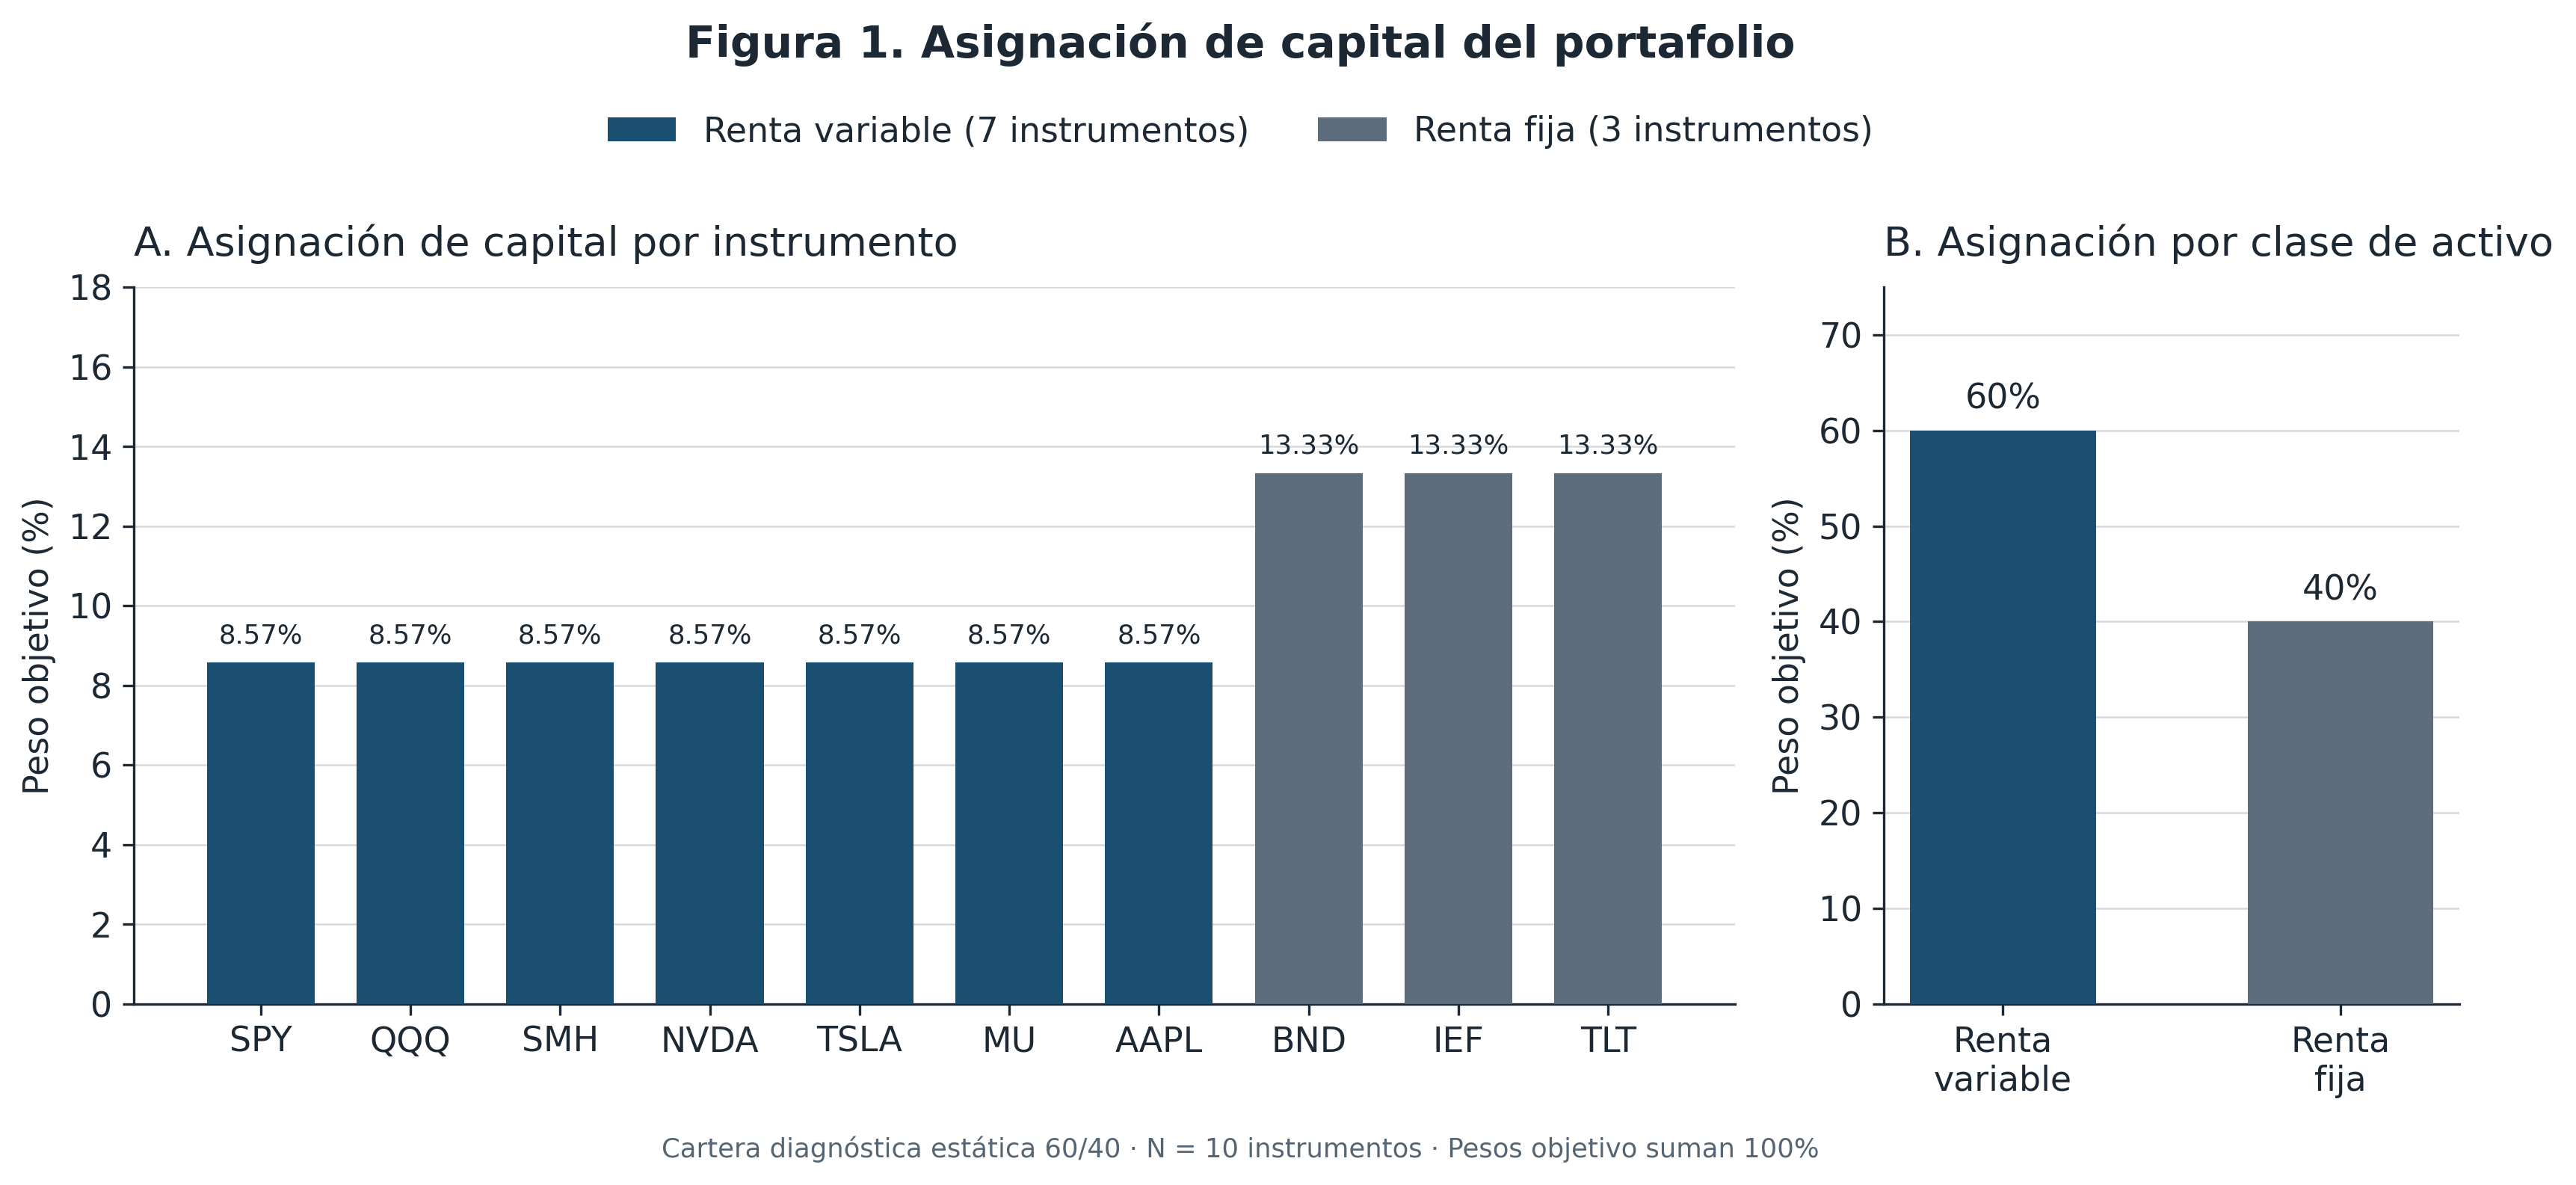
\includegraphics[width=\textwidth]{fig01_portfolio_allocation_es.png}
\caption{Asignación de capital del portafolio --- composición por instrumento y por clase de activo.}
\end{figure}

Desde una perspectiva nominal y de asignación de capital, la cartera presenta múltiples instrumentos y exposición conjunta a renta variable y renta fija. En esta etapa aún no se evalúa si dicha estructura implica diversificación efectiva.

% ========================= 3. PESOS =========================
\section{Primera capa del diagnóstico: \textquestiondown{}cuántos activos tenemos?}

\paragraph{Pregunta.}
\textquestiondown{}El número nominal de instrumentos describe adecuadamente la dispersión del capital?

El punto de partida es el número nominal de posiciones:
\[
N=10.
\]
El conteo de activos no identifica concentraciones derivadas de la distribución de los pesos. Se utiliza el índice de Herfindahl--Hirschman
\[
\mathrm{HHI}=\sum_{i=1}^{N} w_i^{2},
\]
y el número efectivo de posiciones por capital
\[
N_{\mathrm{eff,weights}}=\frac{1}{\sum_{i=1}^{N} w_i^{2}}=\frac{1}{\mathrm{HHI}},
\]
que expresa el número de posiciones equiponderadas que producirían un grado equivalente de concentración del capital.

\begin{table}[H]
\centering
\small
\begin{tabular}{lc}
\toprule
Métrica & Valor \\
\midrule
Número nominal de activos \(N\) & 10 \\
HHI & 0{,}1048 \\
\(N_{\mathrm{eff,weights}}\) & 9{,}55 \\
\bottomrule
\end{tabular}
\caption{Concentración de capital a partir de pesos objetivo.}
\end{table}

\begin{figure}[H]
\centering
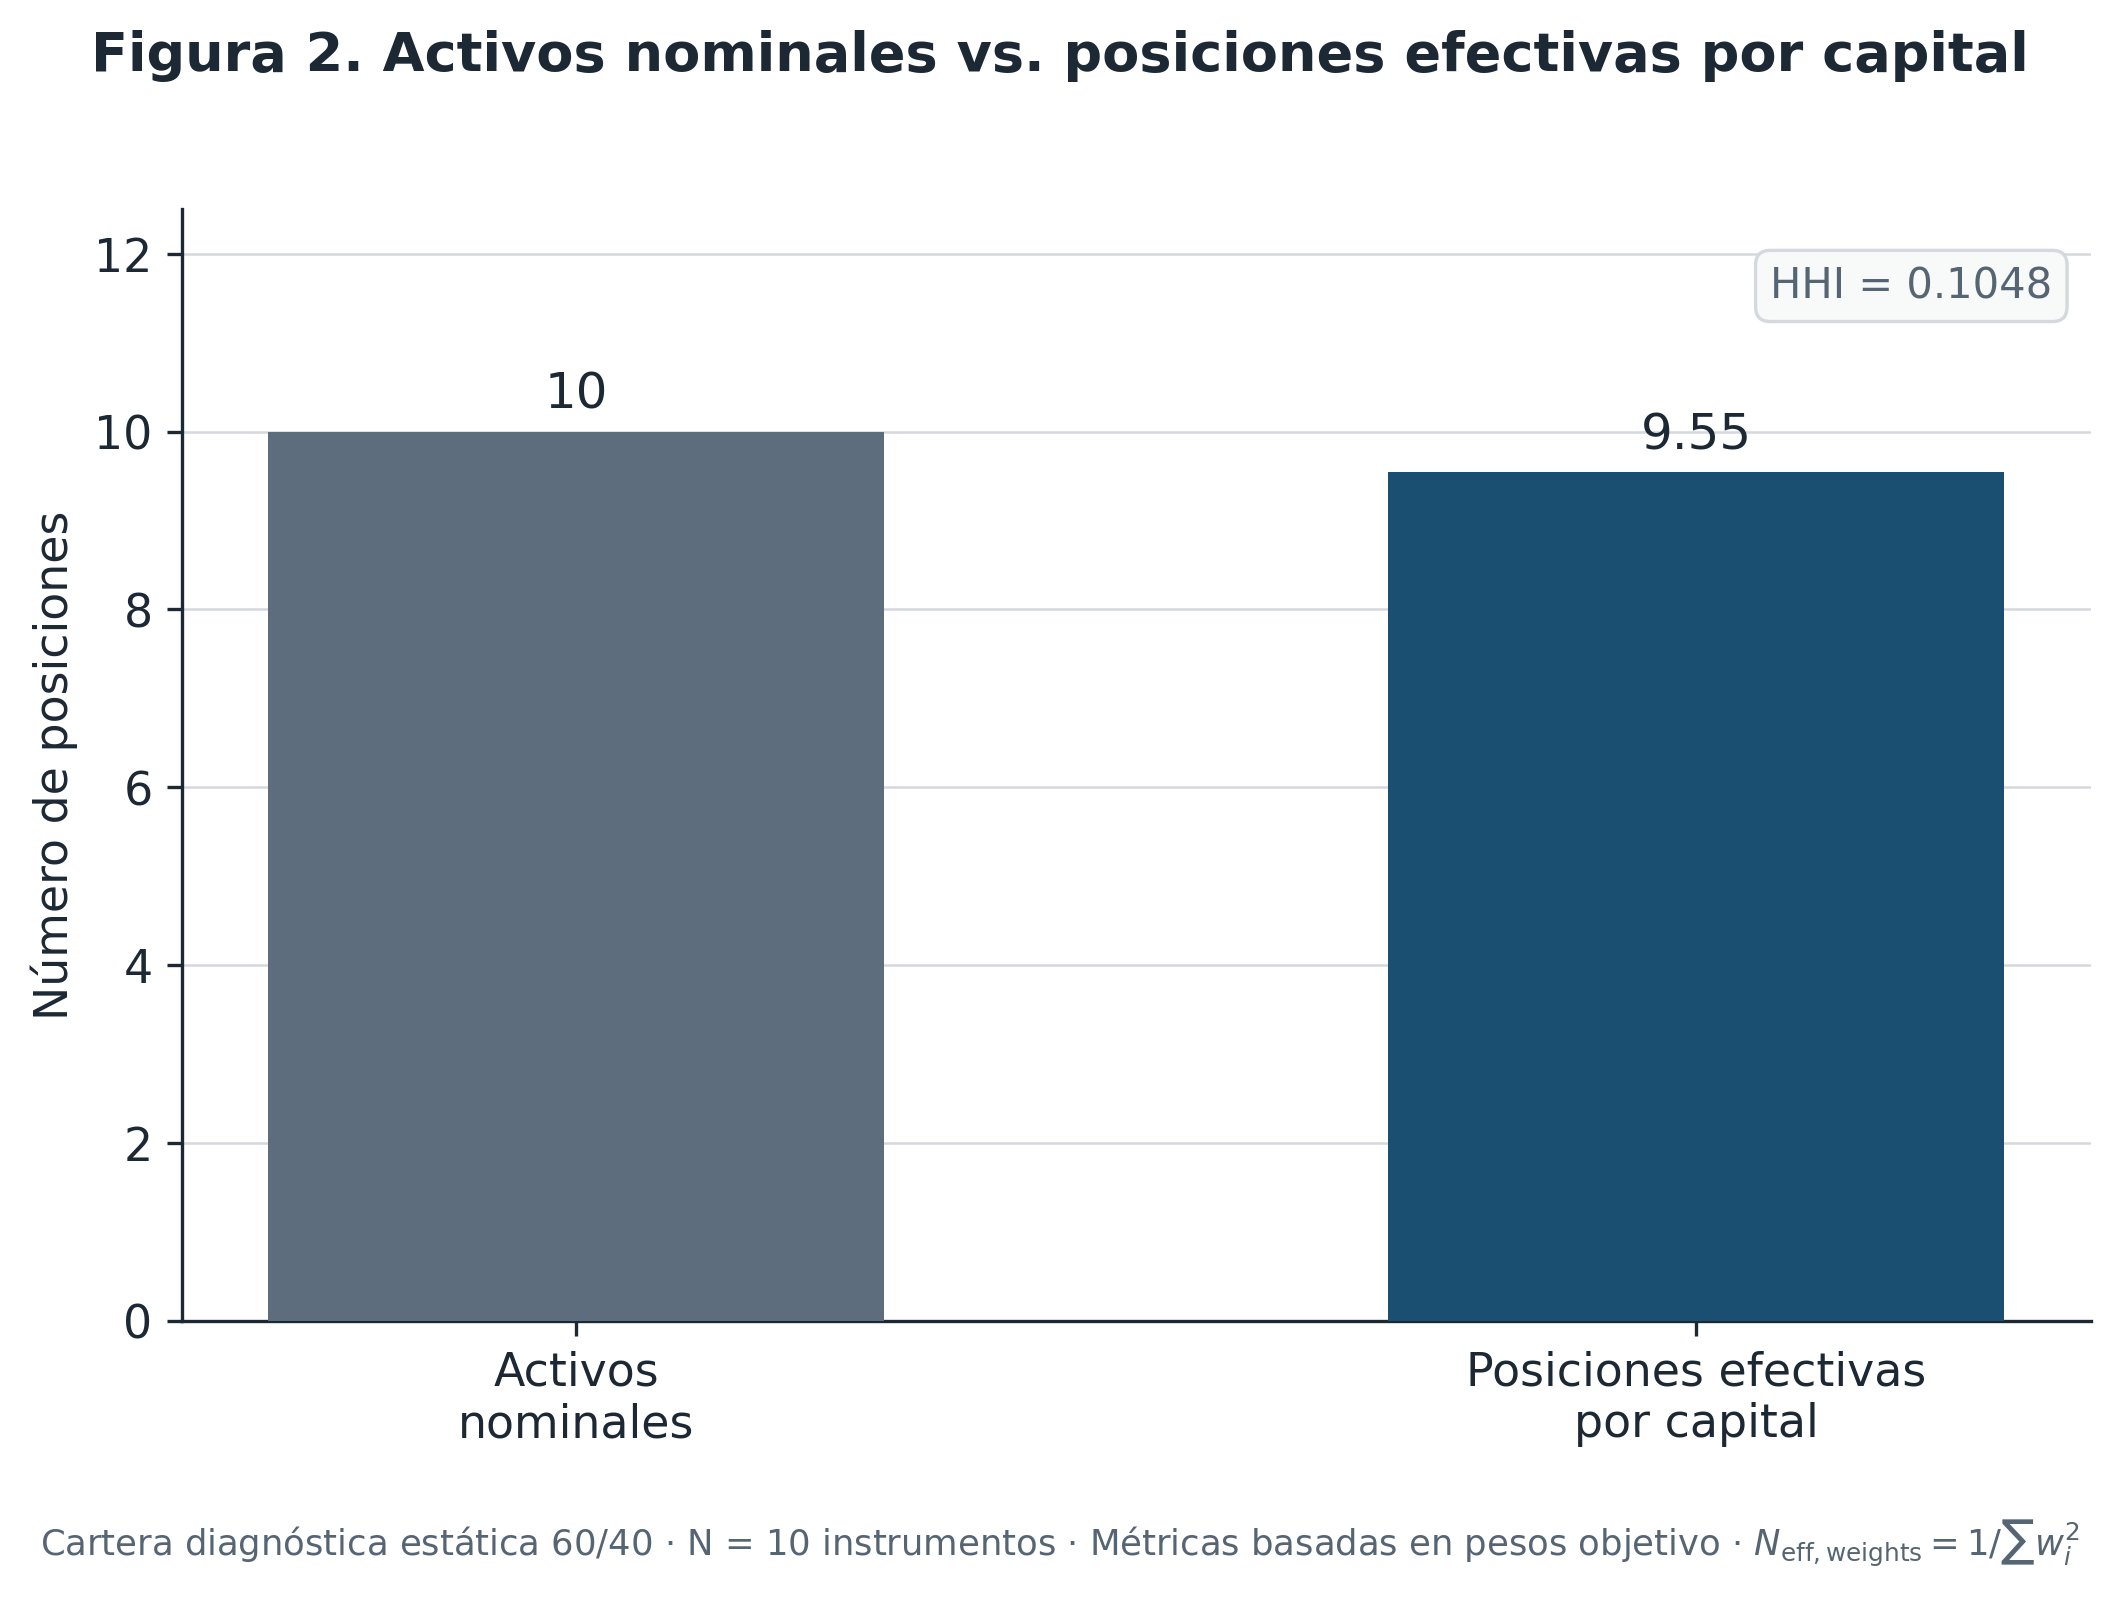
\includegraphics[width=0.78\textwidth]{fig02_effective_positions_capital_es.png}
\caption{Activos nominales vs.\ posiciones efectivas por capital.}
\end{figure}

Los resultados muestran que, desde la perspectiva de la asignación de capital, el portafolio presenta una elevada dispersión. Las diez posiciones nominales equivalen a 9{,}55 posiciones equiponderadas efectivas, una diferencia reducida explicada por el mayor peso individual de los tres instrumentos de renta fija (13{,}33\%) frente a cada posición de renta variable (8{,}57\%). Por lo tanto, no se observa una concentración significativa del capital derivada de los pesos objetivo. Esta primera aproximación no incorpora la dependencia entre retornos ni la contribución de cada activo al riesgo total.

% ========================= 4. DEPENDENCIA =========================
\section{Segunda capa del diagnóstico: \textquestiondown{}cómo se mueven los activos?}

\paragraph{Pregunta.}
\textquestiondown{}Diez instrumentos representan diez comportamientos independientes?

Se estiman correlaciones de Pearson sobre retornos logarítmicos diarios (\(T=2{,}636\) observaciones).

\begin{table}[H]
\centering
\small
\begin{tabular}{lc}
\toprule
Métrica & Valor \\
\midrule
Correlación media (pares off-diagonal) & 0{,}34 \\
Media intra--renta variable & 0{,}63 \\
Media intra--renta fija & 0{,}86 \\
Media entre clases & $-0{,}03$ \\
Mínimo / máximo entre pares & $-0{,}16$ / $0{,}93$ \\
Enlaces con \(\lvert\rho\rvert\ge 0{,}60\) & 15 \\
\bottomrule
\end{tabular}
\caption{Resumen de la estructura de dependencia.}
\end{table}

\begin{figure}[H]
\centering
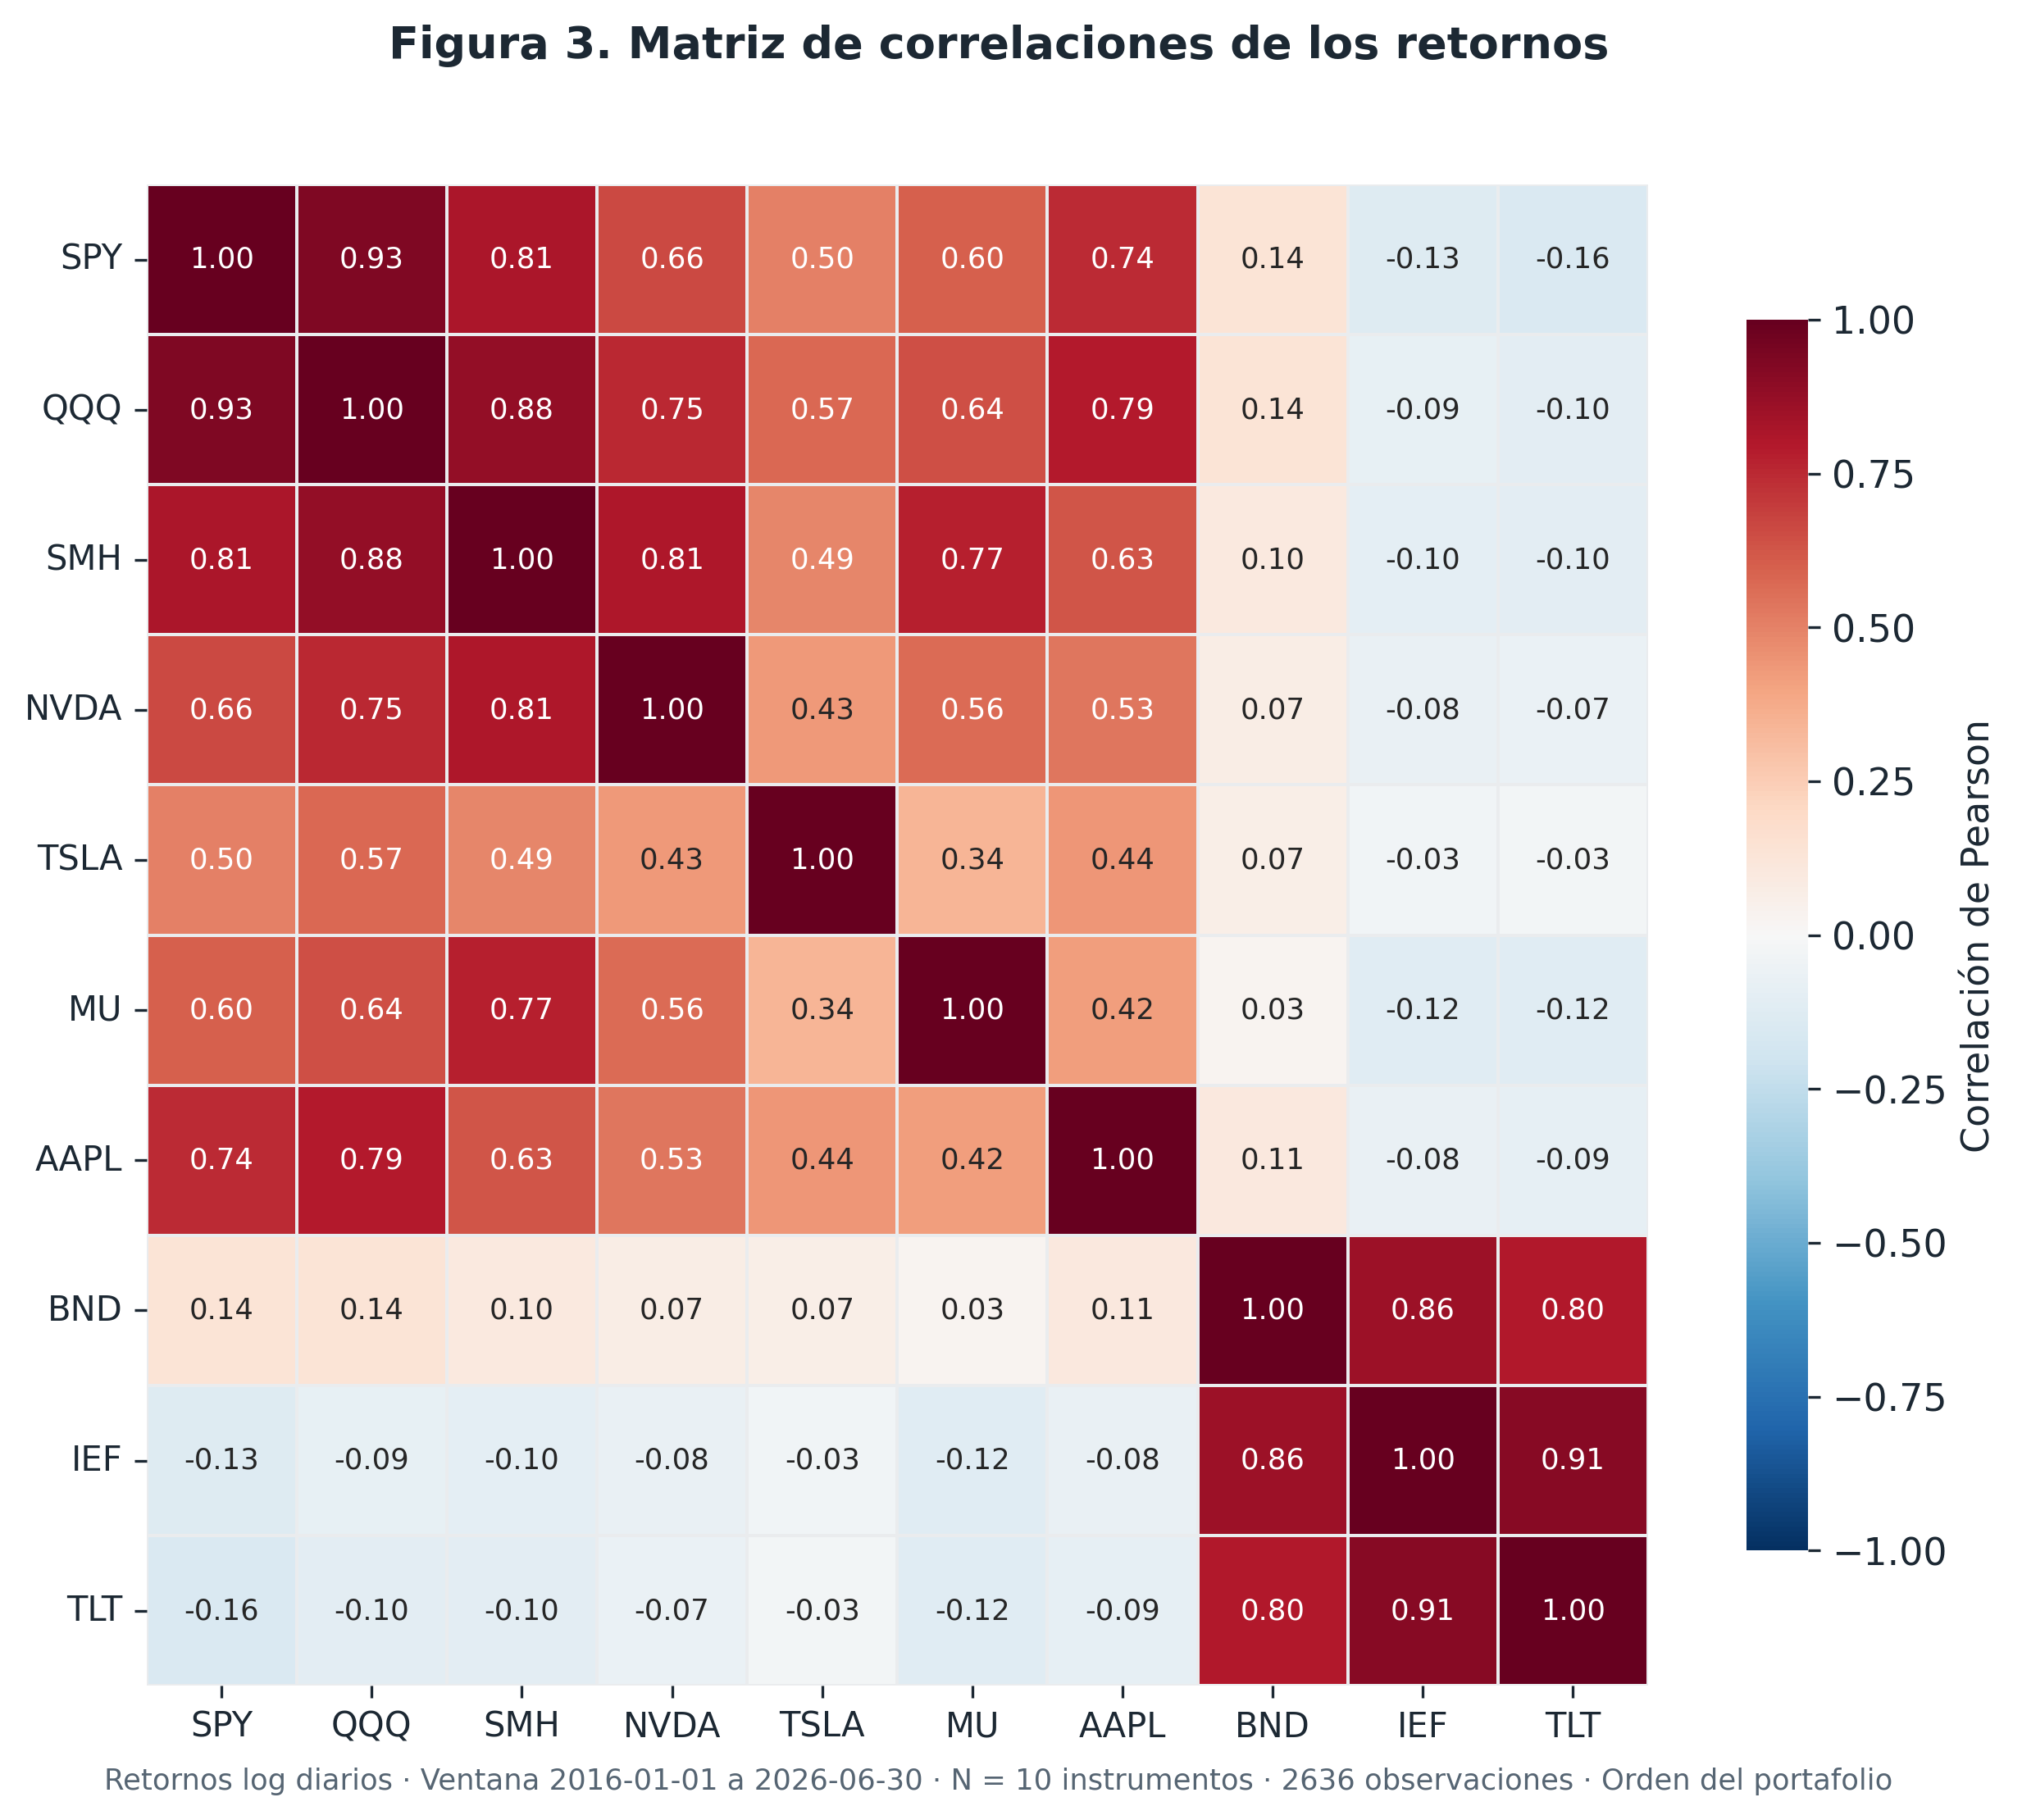
\includegraphics[width=0.92\textwidth]{fig03_correlation_heatmap_es.png}
\caption{Matriz de correlaciones de los retornos.}
\end{figure}

\begin{figure}[H]
\centering
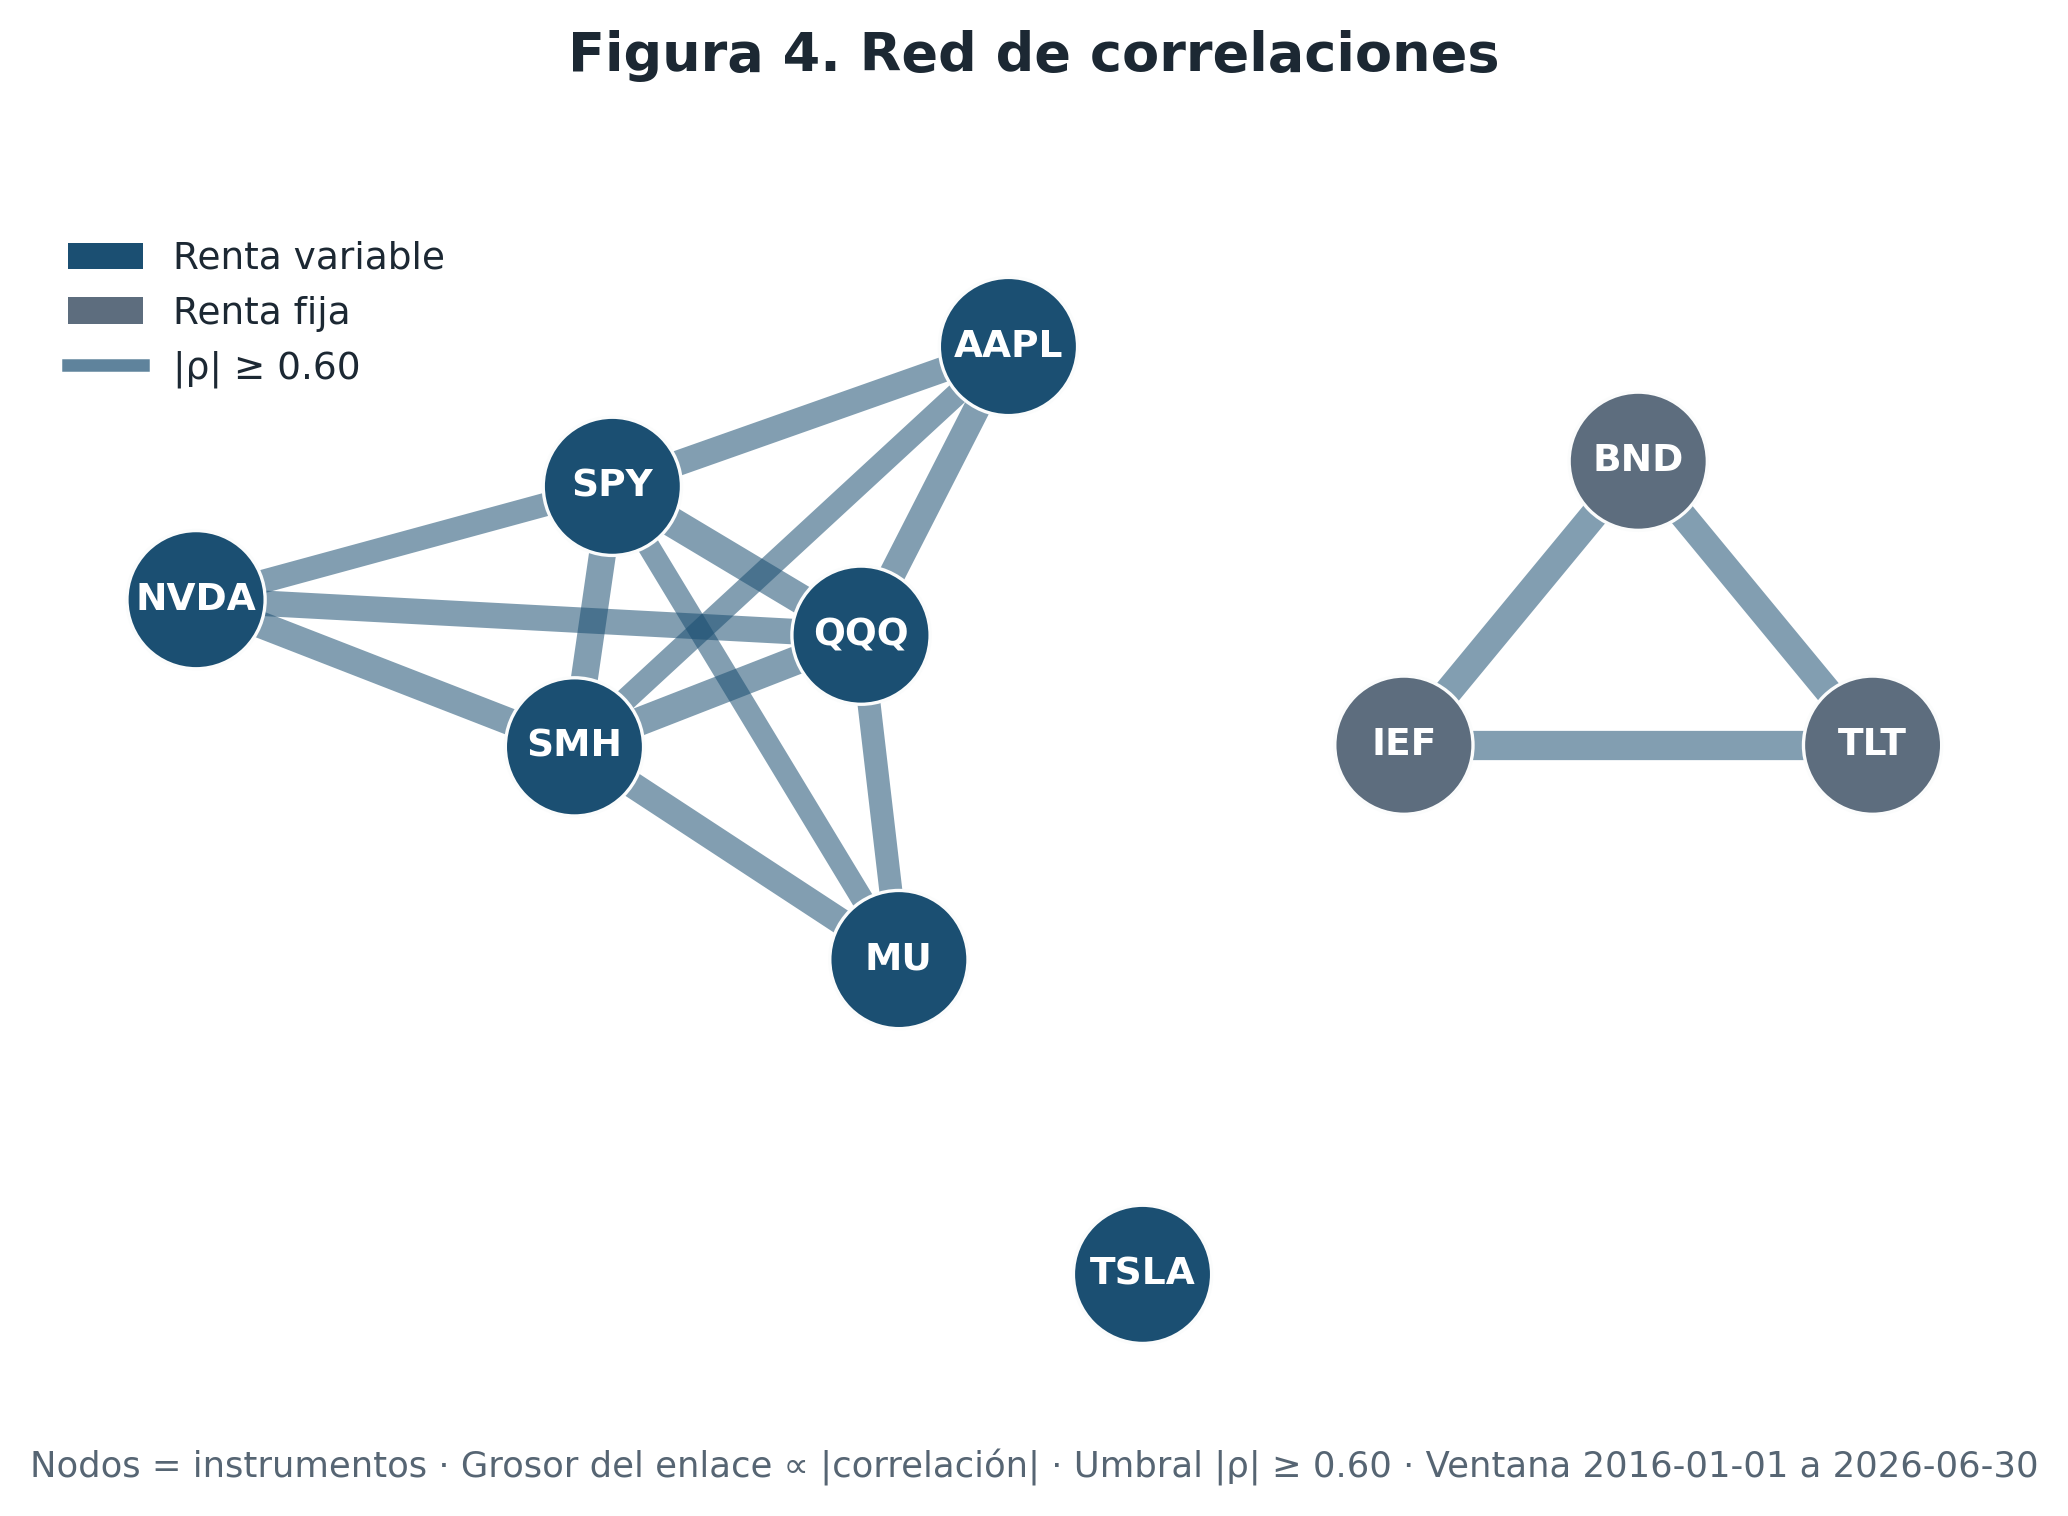
\includegraphics[width=0.88\textwidth]{fig04_correlation_network_es.png}
\caption{Red de correlaciones (\(\lvert\rho\rvert\ge 0{,}60\)).}
\end{figure}

La matriz presenta la evidencia cuantitativa completa de la dependencia; la red sintetiza las conexiones más intensas bajo un umbral predefinido. Se observan dos bloques de dependencia elevada (renta variable y renta fija) y correlaciones cruzadas cercanas a cero. TSLA permanece aislado en la red bajo el umbral \(\lvert\rho\rvert\ge 0{,}60\): ello indica únicamente que no alcanza dicho umbral con el resto del universo en la muestra, sin interpretarlo automáticamente como fuente independiente de riesgo. En conjunto, diez instrumentos no equivalen a diez comportamientos independientes.

% ========================= 5. RIESGO =========================
\section{Tercera capa del diagnóstico: \textquestiondown{}quién genera realmente el riesgo?}

\paragraph{Pregunta.}
\textquestiondown{}Una cartera 60/40 por capital también es 60/40 por riesgo?

Con pesos objetivo constantes \(w\) y covarianza muestral \(\Sigma\),
\[
\sigma_p=\sqrt{w^{\top}\Sigma w},\quad
\mathrm{MRC}_i=\frac{(\Sigma w)_i}{\sigma_p},\quad
\mathrm{RC}_i=w_i\,\mathrm{MRC}_i,\quad
\mathrm{PRC}_i=\frac{\mathrm{RC}_i}{\sigma_p}.
\]
La identidad de Euler implica \(\sum_i \mathrm{RC}_i=\sigma_p\) y \(\sum_i\mathrm{PRC}_i=1\).

\begin{table}[H]
\centering
\small
\begin{tabular}{lcc}
\toprule
Clase & Capital & Riesgo (\(\sum\) PRC) \\
\midrule
Renta variable & 60{,}0\% & 97{,}65\% \\
Renta fija & 40{,}0\% & 2{,}35\% \\
\bottomrule
\end{tabular}
\caption{Asignación de capital vs.\ contribución al riesgo por clase.}
\end{table}

\begin{figure}[H]
\centering
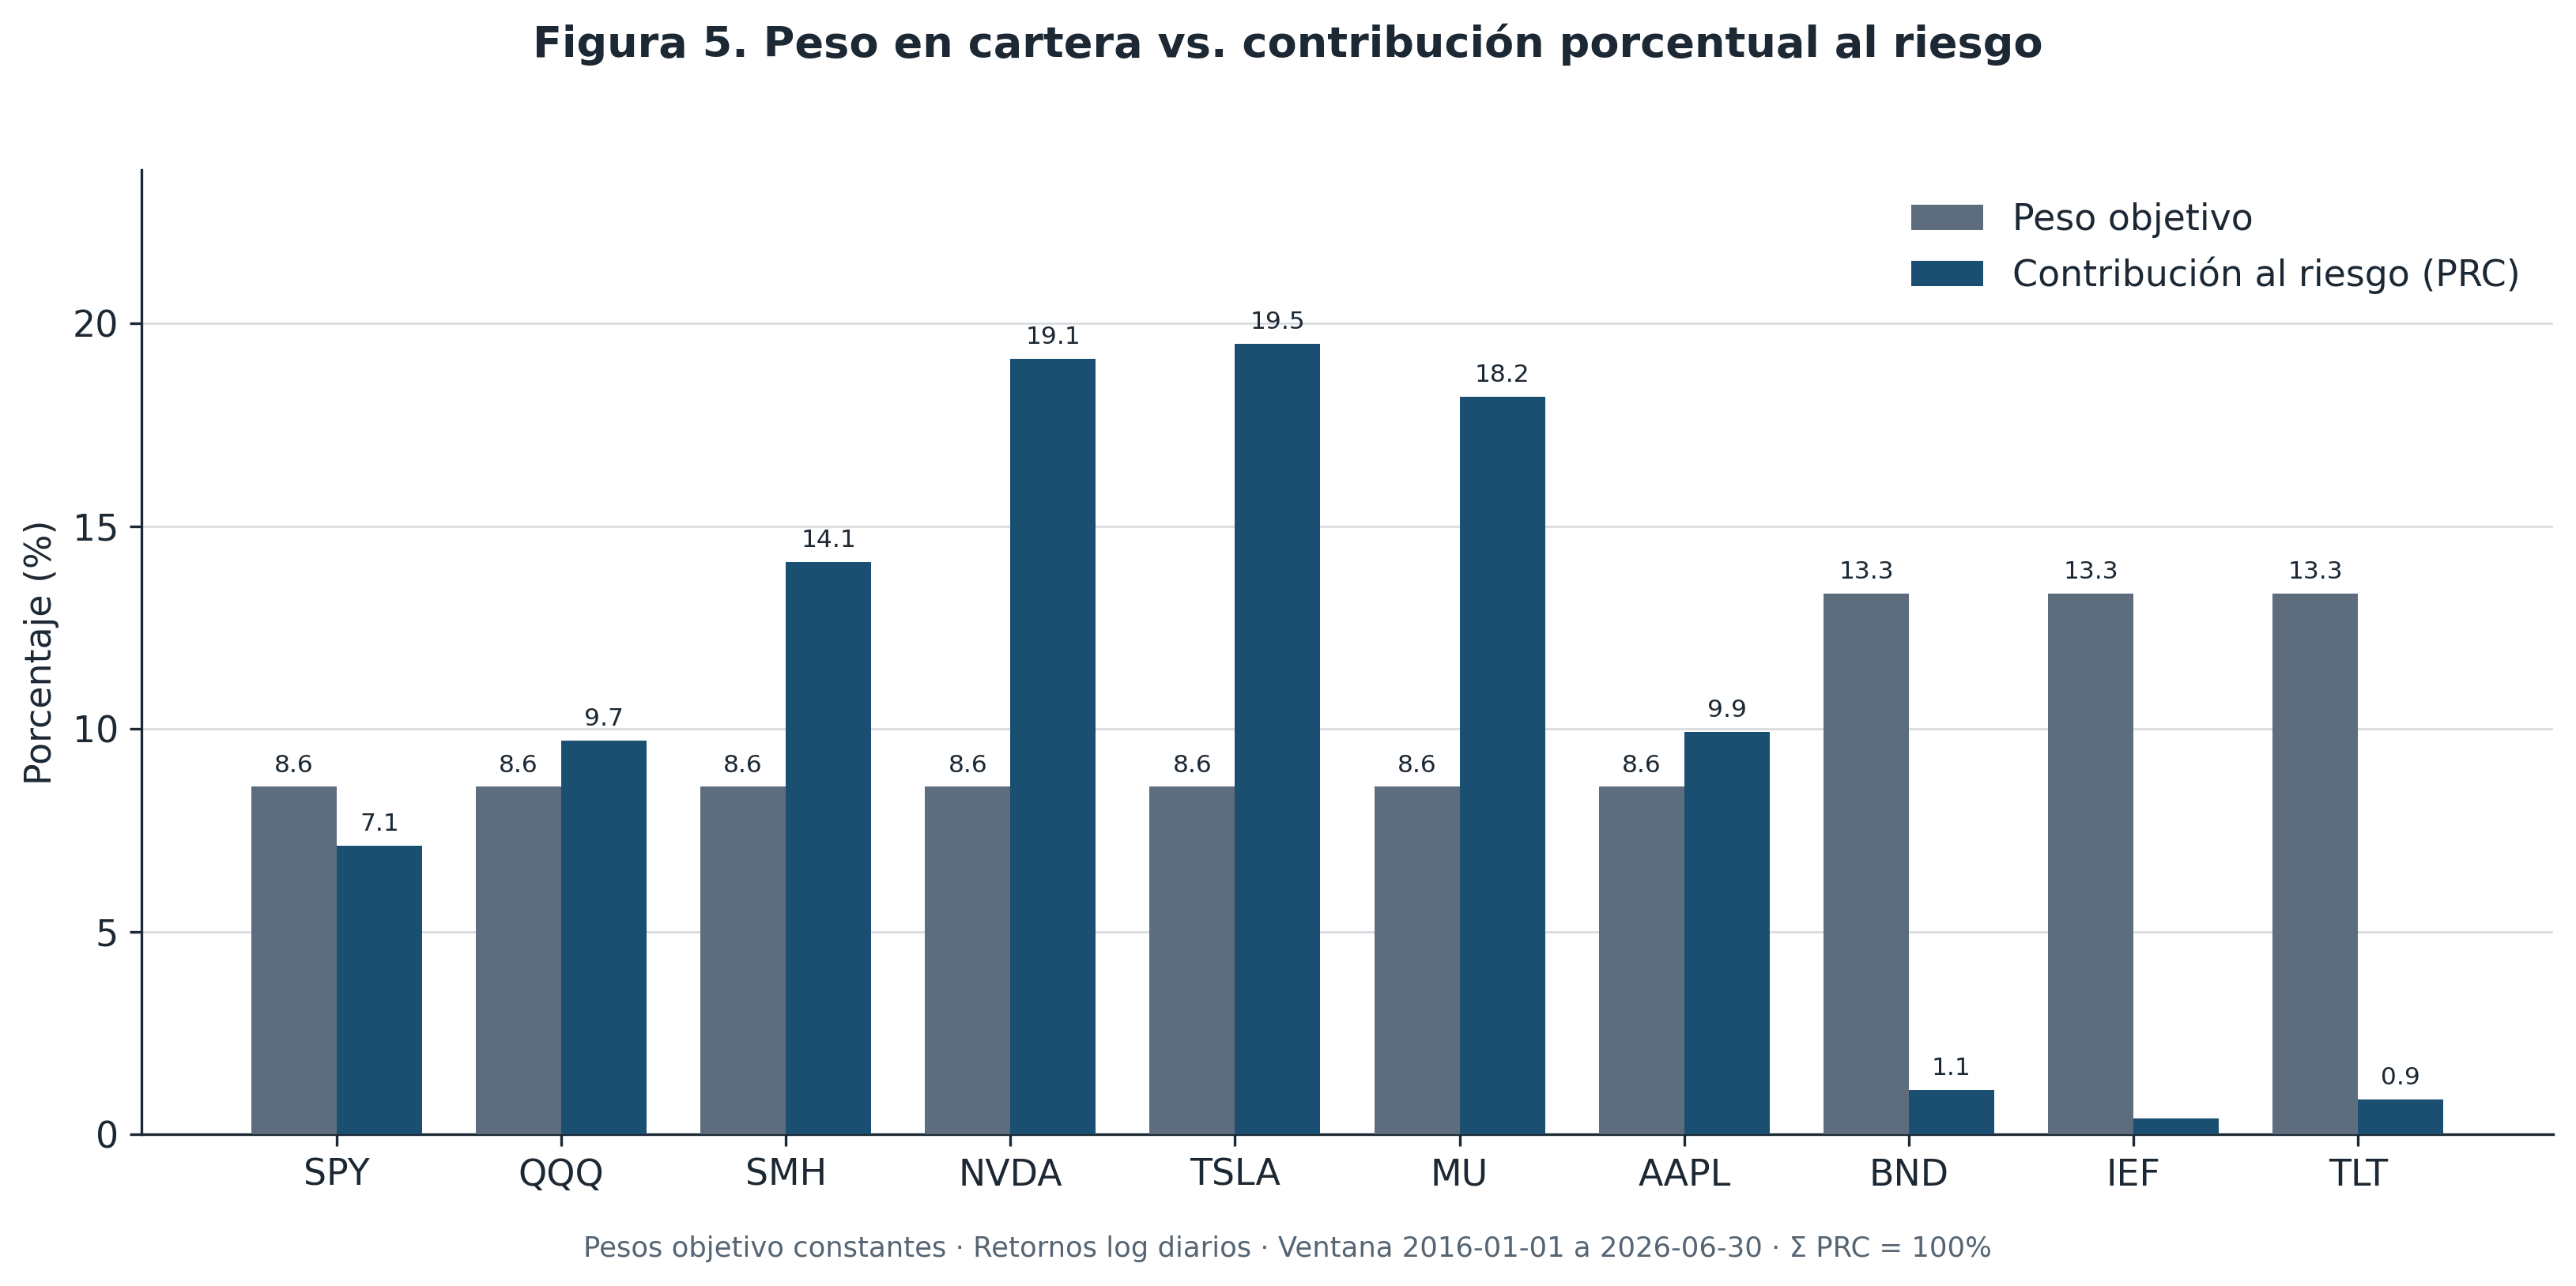
\includegraphics[width=\textwidth]{fig05_weight_vs_prc_es.png}
\caption{Peso en cartera vs.\ contribución porcentual al riesgo.}
\end{figure}

\begin{figure}[H]
\centering
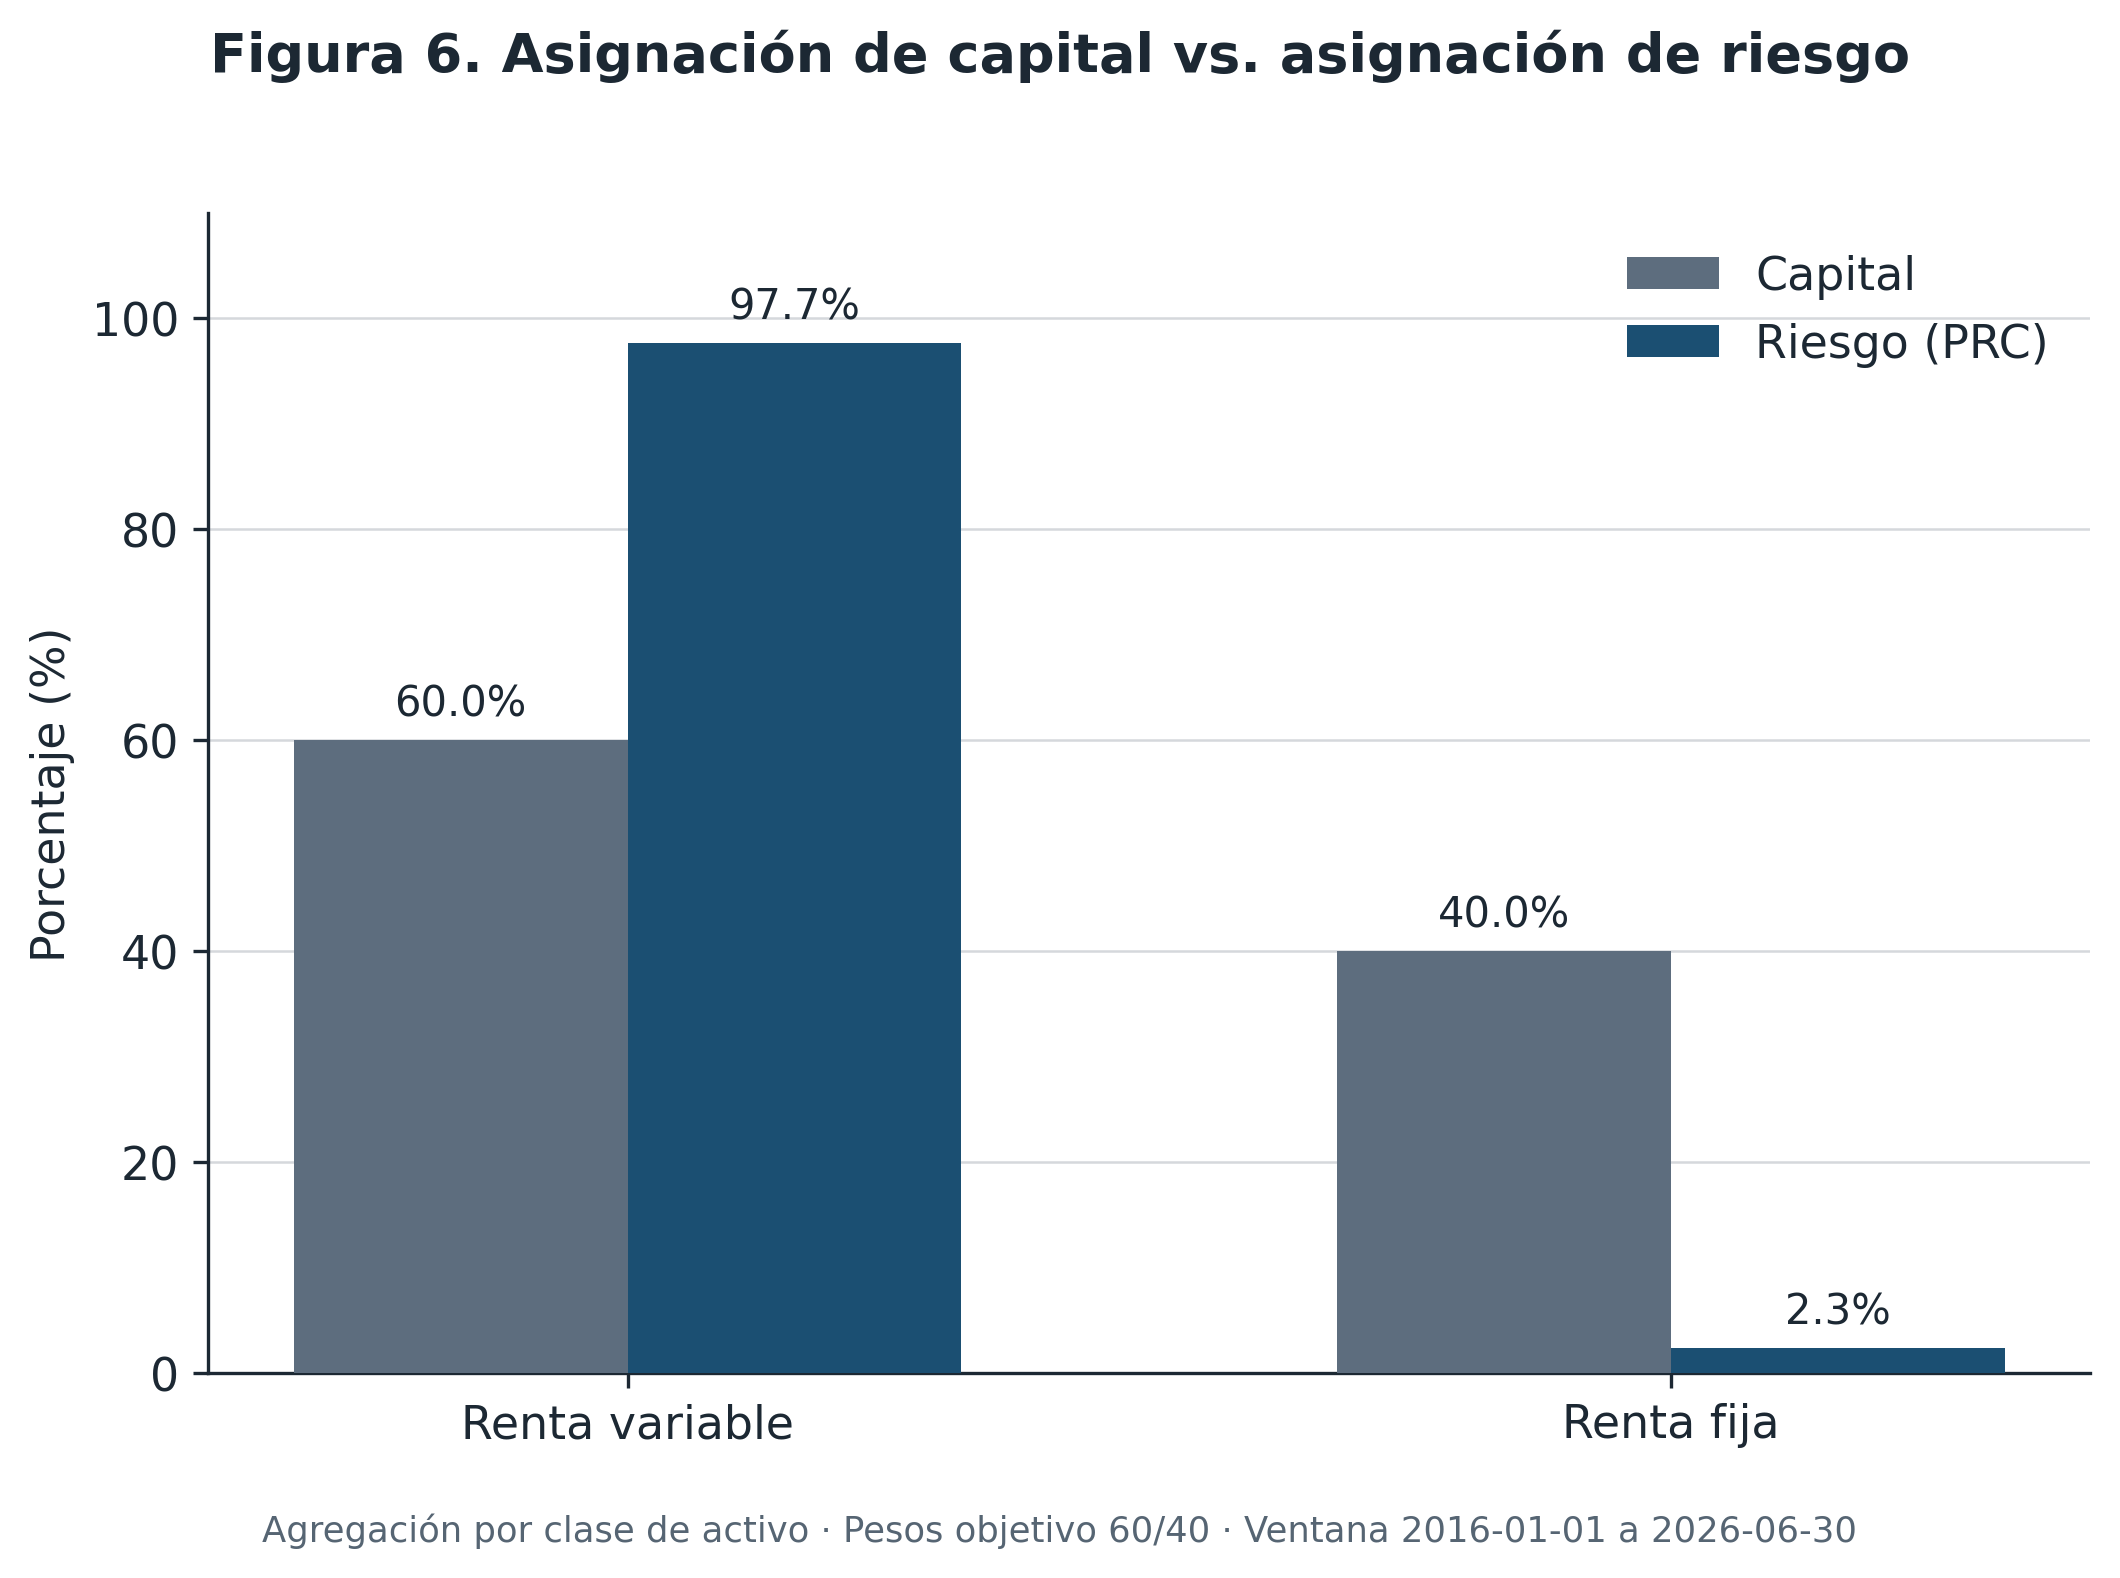
\includegraphics[width=0.78\textwidth]{fig06_capital_vs_risk_allocation_es.png}
\caption{Asignación de capital vs.\ asignación de riesgo.}
\end{figure}

Los resultados muestran una marcada disociación entre la asignación de capital y la distribución de las contribuciones al riesgo. Aunque el 60\% del capital se encuentra asignado a renta variable, los instrumentos de esta clase concentran el 97{,}65\% de la contribución total al riesgo. En contraste, el bloque de renta fija (40\% del capital) concentra únicamente el 2{,}35\% de la contribución estimada mediante la descomposición de Euler.

La divergencia también es significativa a nivel de instrumento. TSLA, NVDA y MU reciben el mismo peso objetivo que el resto de la renta variable ---8{,}57\%---, pero sus PRC alcanzan 19{,}49\%, 19{,}12\% y 18{,}18\%, respectivamente. SPY contribuye un 7{,}12\% del riesgo total con idéntica asignación de capital. En la muestra analizada, la clasificación 60/40 describe la estructura nominal de capital, pero no su estructura de riesgo.

% ========================= 6. N EFF =========================
\section{Cuarta capa del diagnóstico: \textquestiondown{}cuántas posiciones efectivas tenemos?}

\paragraph{Pregunta.}
\textquestiondown{}Cuánto se reduce el número de posiciones al pasar del conteo nominal a la concentración del capital y, finalmente, a la del riesgo?

Se comparan
\[
N=10,\qquad
N_{\mathrm{eff,weights}}=\frac{1}{\sum w_i^{2}},\qquad
N_{\mathrm{eff,risk}}=\frac{1}{\sum p_i^{2}},\quad p_i=\mathrm{PRC}_i.
\]

\begin{table}[H]
\centering
\small
\begin{tabular}{lc}
\toprule
Métrica & Valor \\
\midrule
\(N\) & 10 \\
\(N_{\mathrm{eff,weights}}\) & 9{,}55 \\
\(N_{\mathrm{eff,risk}}\) & 6{,}58 \\
\bottomrule
\end{tabular}
\caption{Números efectivos de posiciones.}
\end{table}

\begin{figure}[H]
\centering
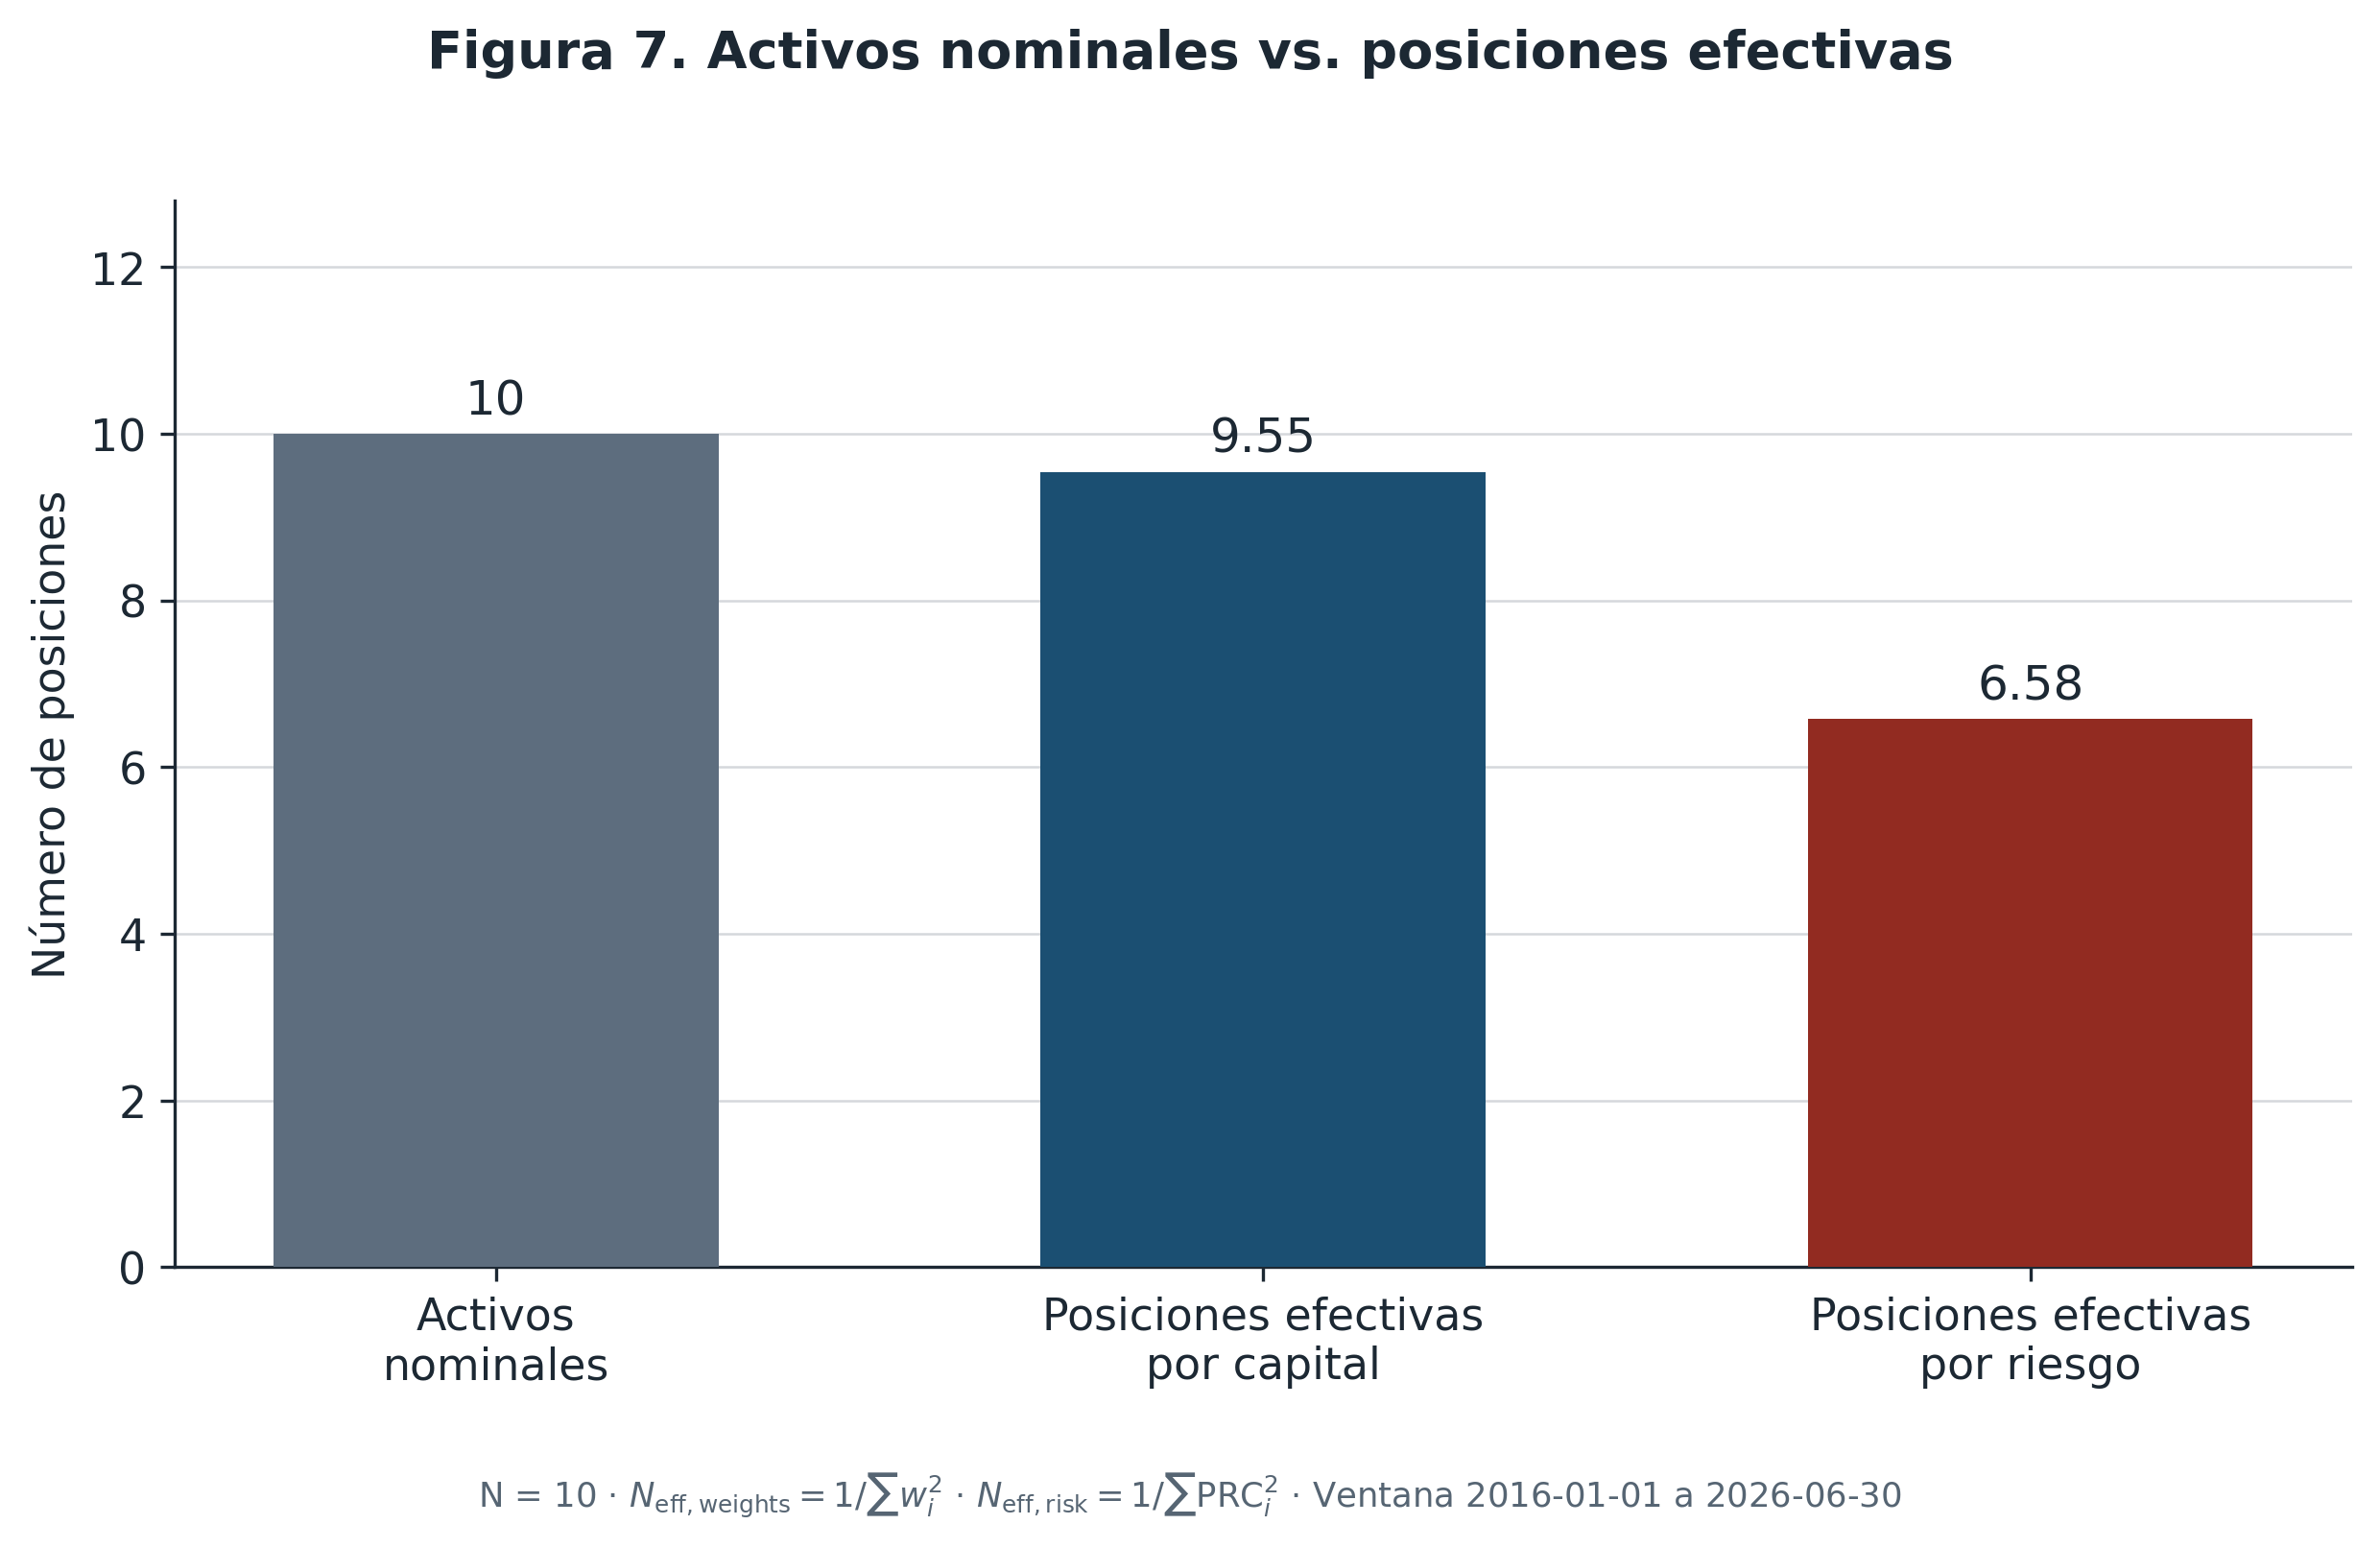
\includegraphics[width=0.82\textwidth]{fig07_effective_positions_es.png}
\caption{Activos nominales vs.\ posiciones efectivas por capital y por riesgo.}
\end{figure}

Desde la perspectiva del capital, las diez posiciones equivalen a 9{,}55 posiciones equiponderadas. Al evaluar la concentración de las contribuciones porcentuales al riesgo, el número efectivo desciende a 6{,}58. En síntesis, el portafolio presenta una elevada dispersión cuando se analiza exclusivamente la asignación de capital; una vez incorporada la distribución de las contribuciones al riesgo, el número efectivo de posiciones se reduce de forma material respecto del conteo nominal.

% ========================= 7. PCA =========================
\section{Quinta capa del diagnóstico: \textquestiondown{}cuántas fuentes comunes de riesgo existen?}

\paragraph{Pregunta.}
\textquestiondown{}Cuántos componentes bastan para explicar la mayor parte de la variabilidad conjunta del portafolio?

Se aplica un PCA sobre la matriz de correlación de los retornos logarítmicos diarios, exclusivamente como herramienta descriptiva de fuentes comunes de variación.

\begin{table}[H]
\centering
\small
\begin{tabular}{lcc}
\toprule
Componente & Varianza explicada & Acumulada \\
\midrule
PC1 & 49{,}29\% & 49{,}29\% \\
PC2 & 27{,}11\% & 76{,}40\% \\
PC3 & 7{,}31\% & 83{,}72\% \\
PC4 & 6{,}06\% & 89{,}78\% \\
PC5 & 4{,}13\% & 93{,}90\% \\
\bottomrule
\end{tabular}
\caption{Varianza explicada por componentes principales.}
\end{table}

\begin{table}[H]
\centering
\small
\begin{tabular}{lc}
\toprule
Umbral & Componentes necesarios \\
\midrule
\(\ge 80\%\) & 3 \\
\(\ge 90\%\) & 5 \\
\bottomrule
\end{tabular}
\caption{Número de componentes para umbrales de varianza acumulada.}
\end{table}

\begin{figure}[H]
\centering
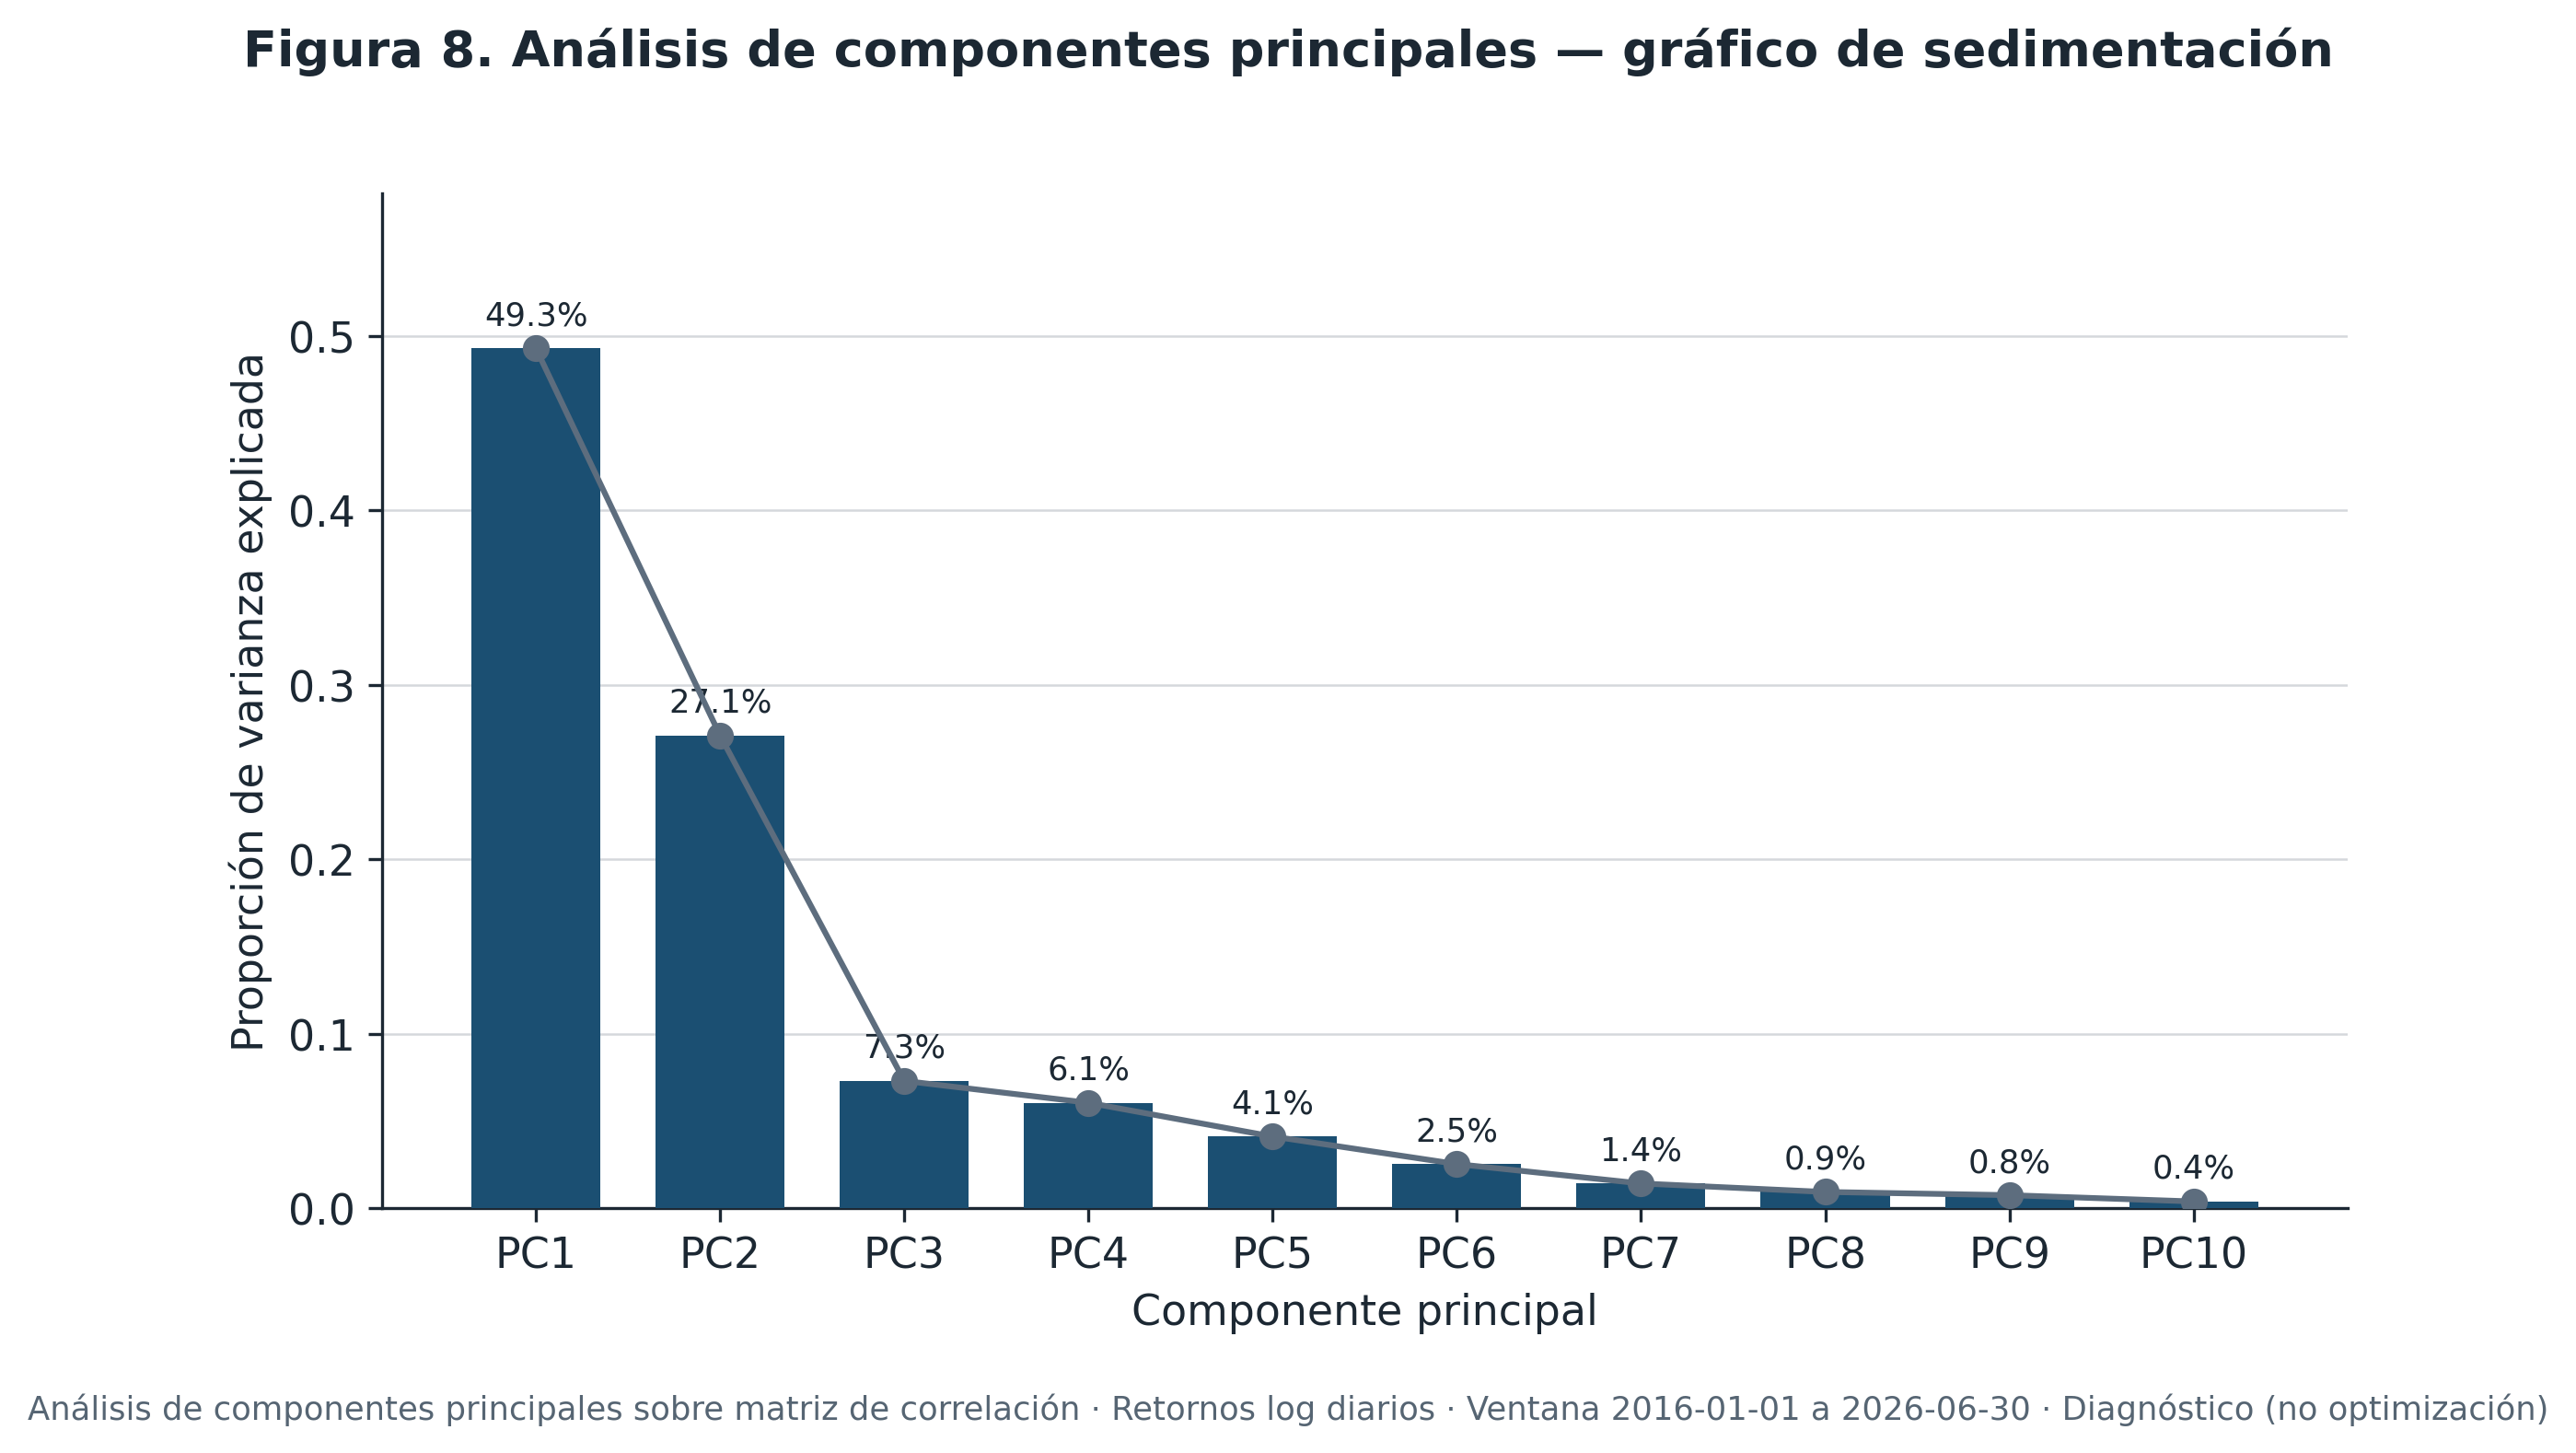
\includegraphics[width=0.85\textwidth]{fig08_pca_scree_es.png}
\caption{PCA --- gráfico de sedimentación (scree).}
\end{figure}

\begin{figure}[H]
\centering
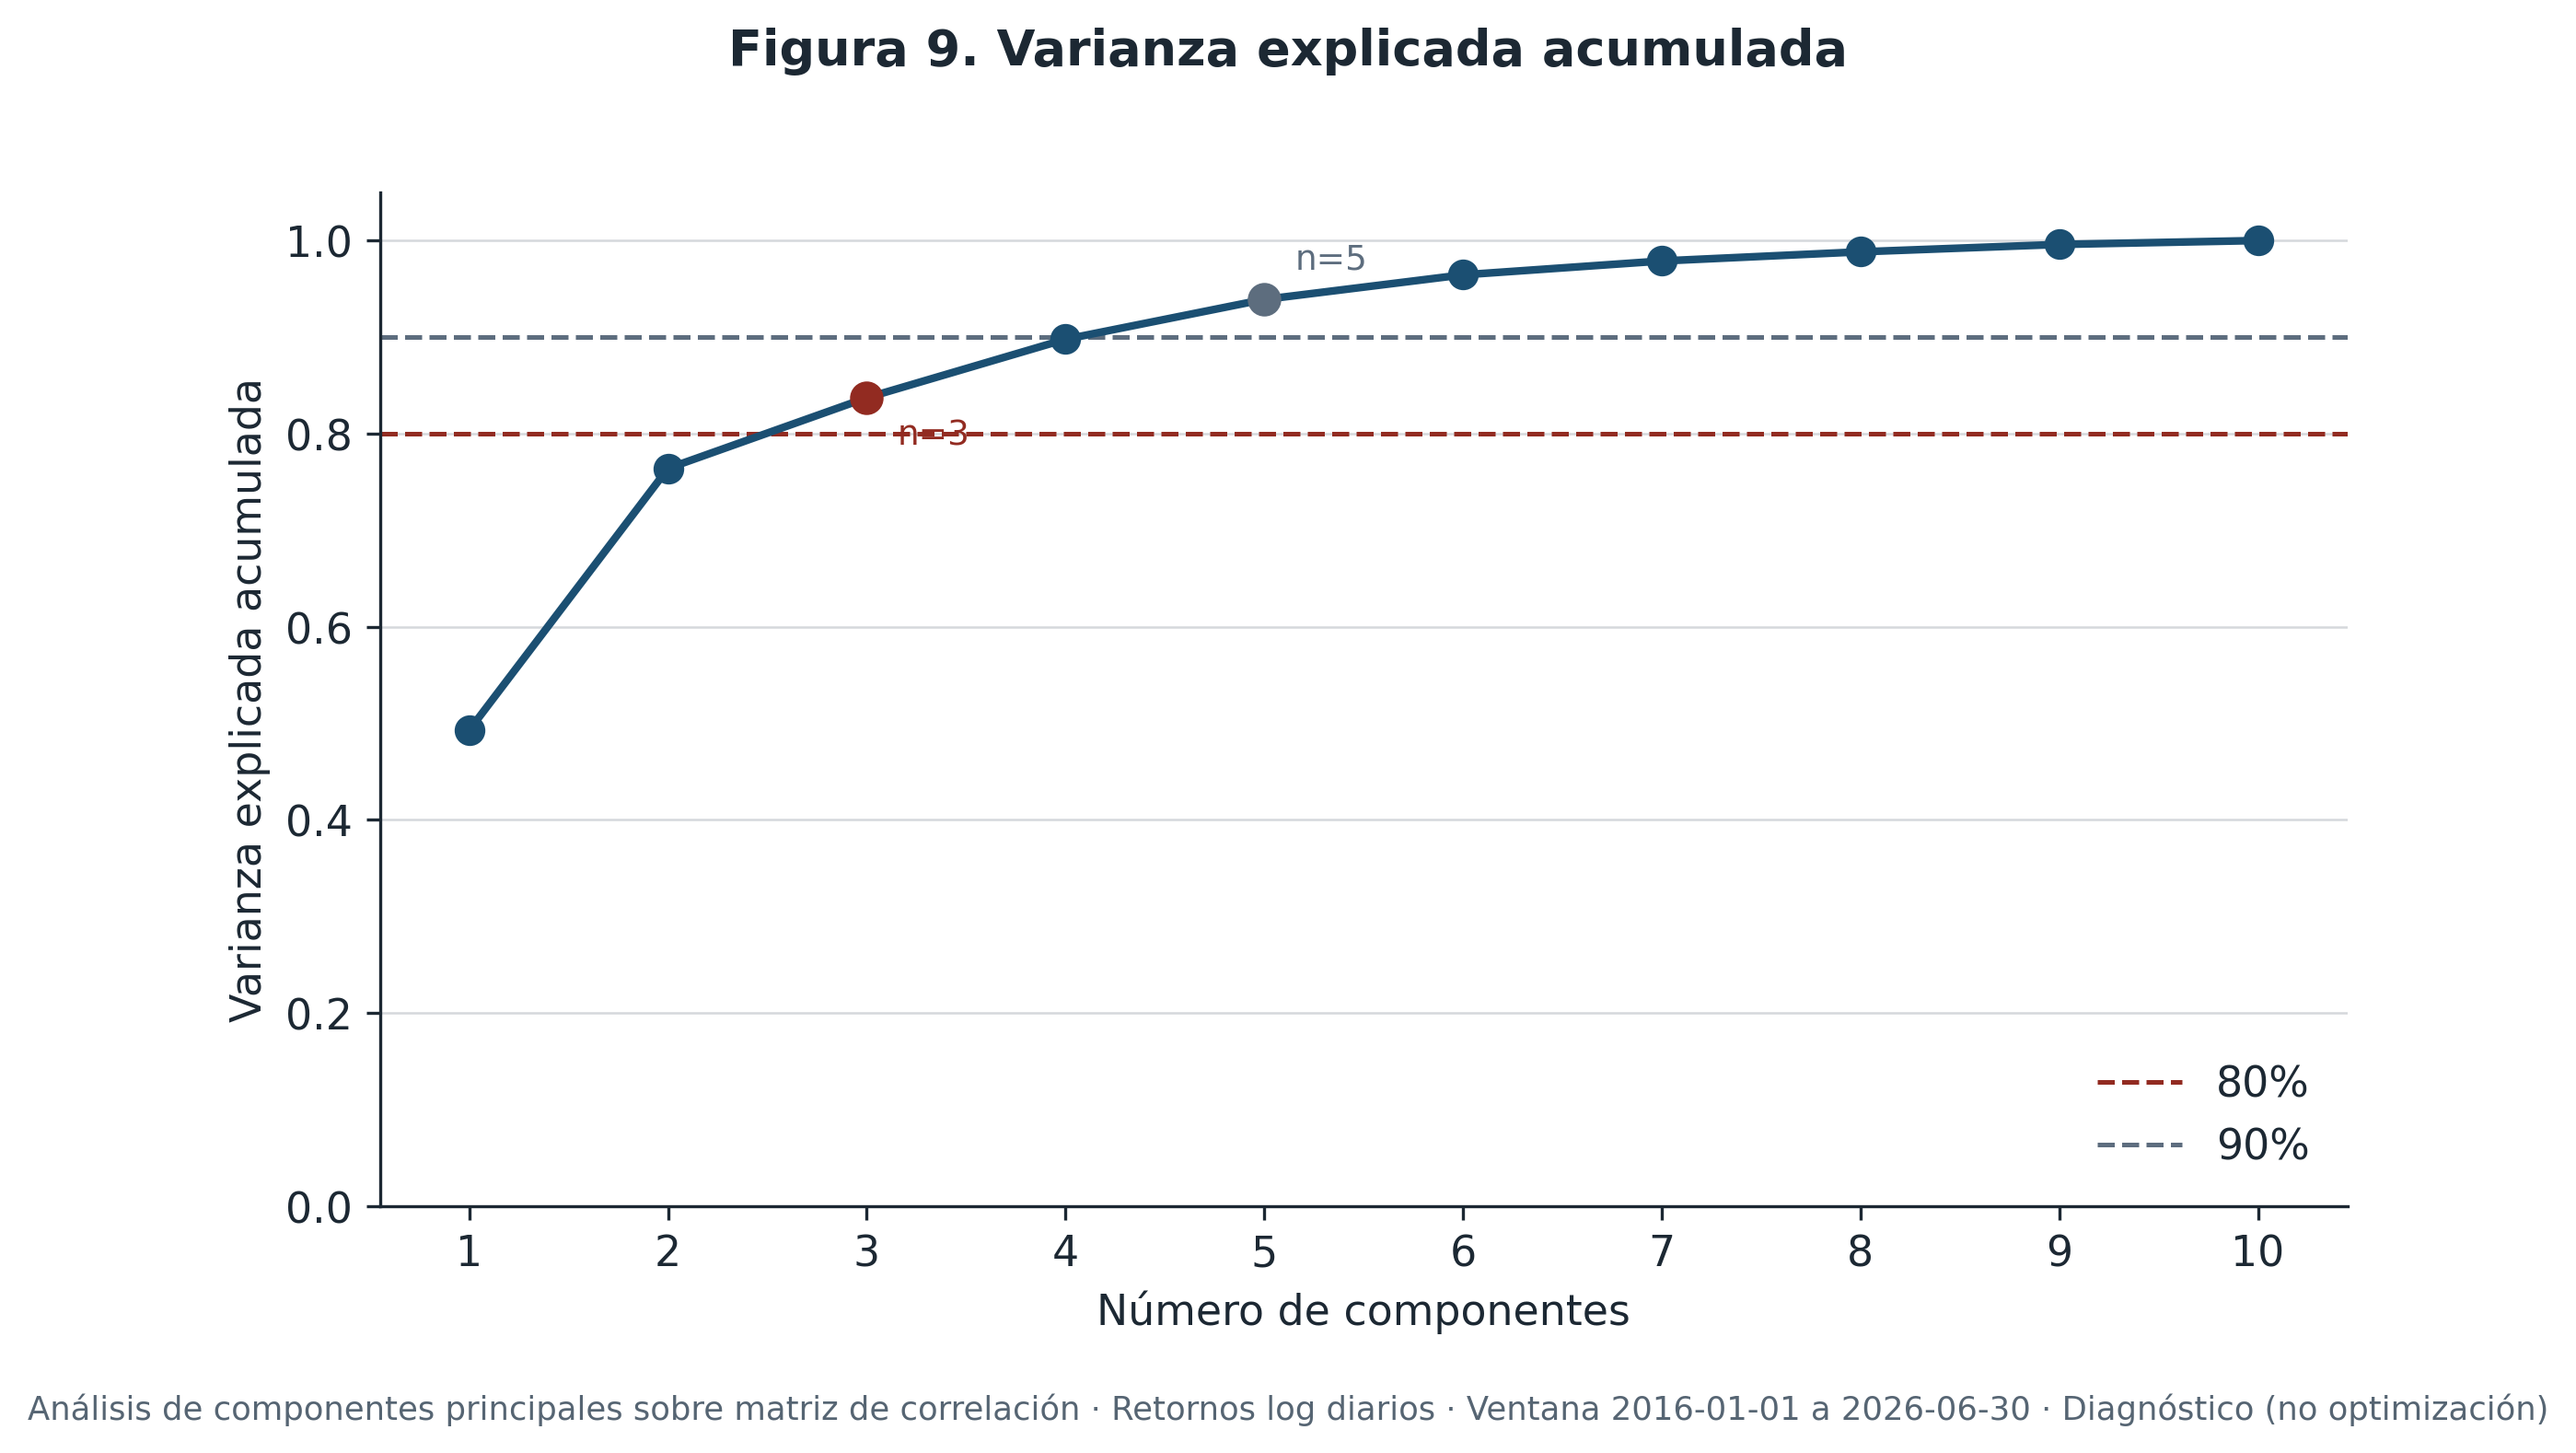
\includegraphics[width=0.85\textwidth]{fig09_pca_cumulative_es.png}
\caption{Varianza explicada acumulada.}
\end{figure}

\begin{figure}[H]
\centering
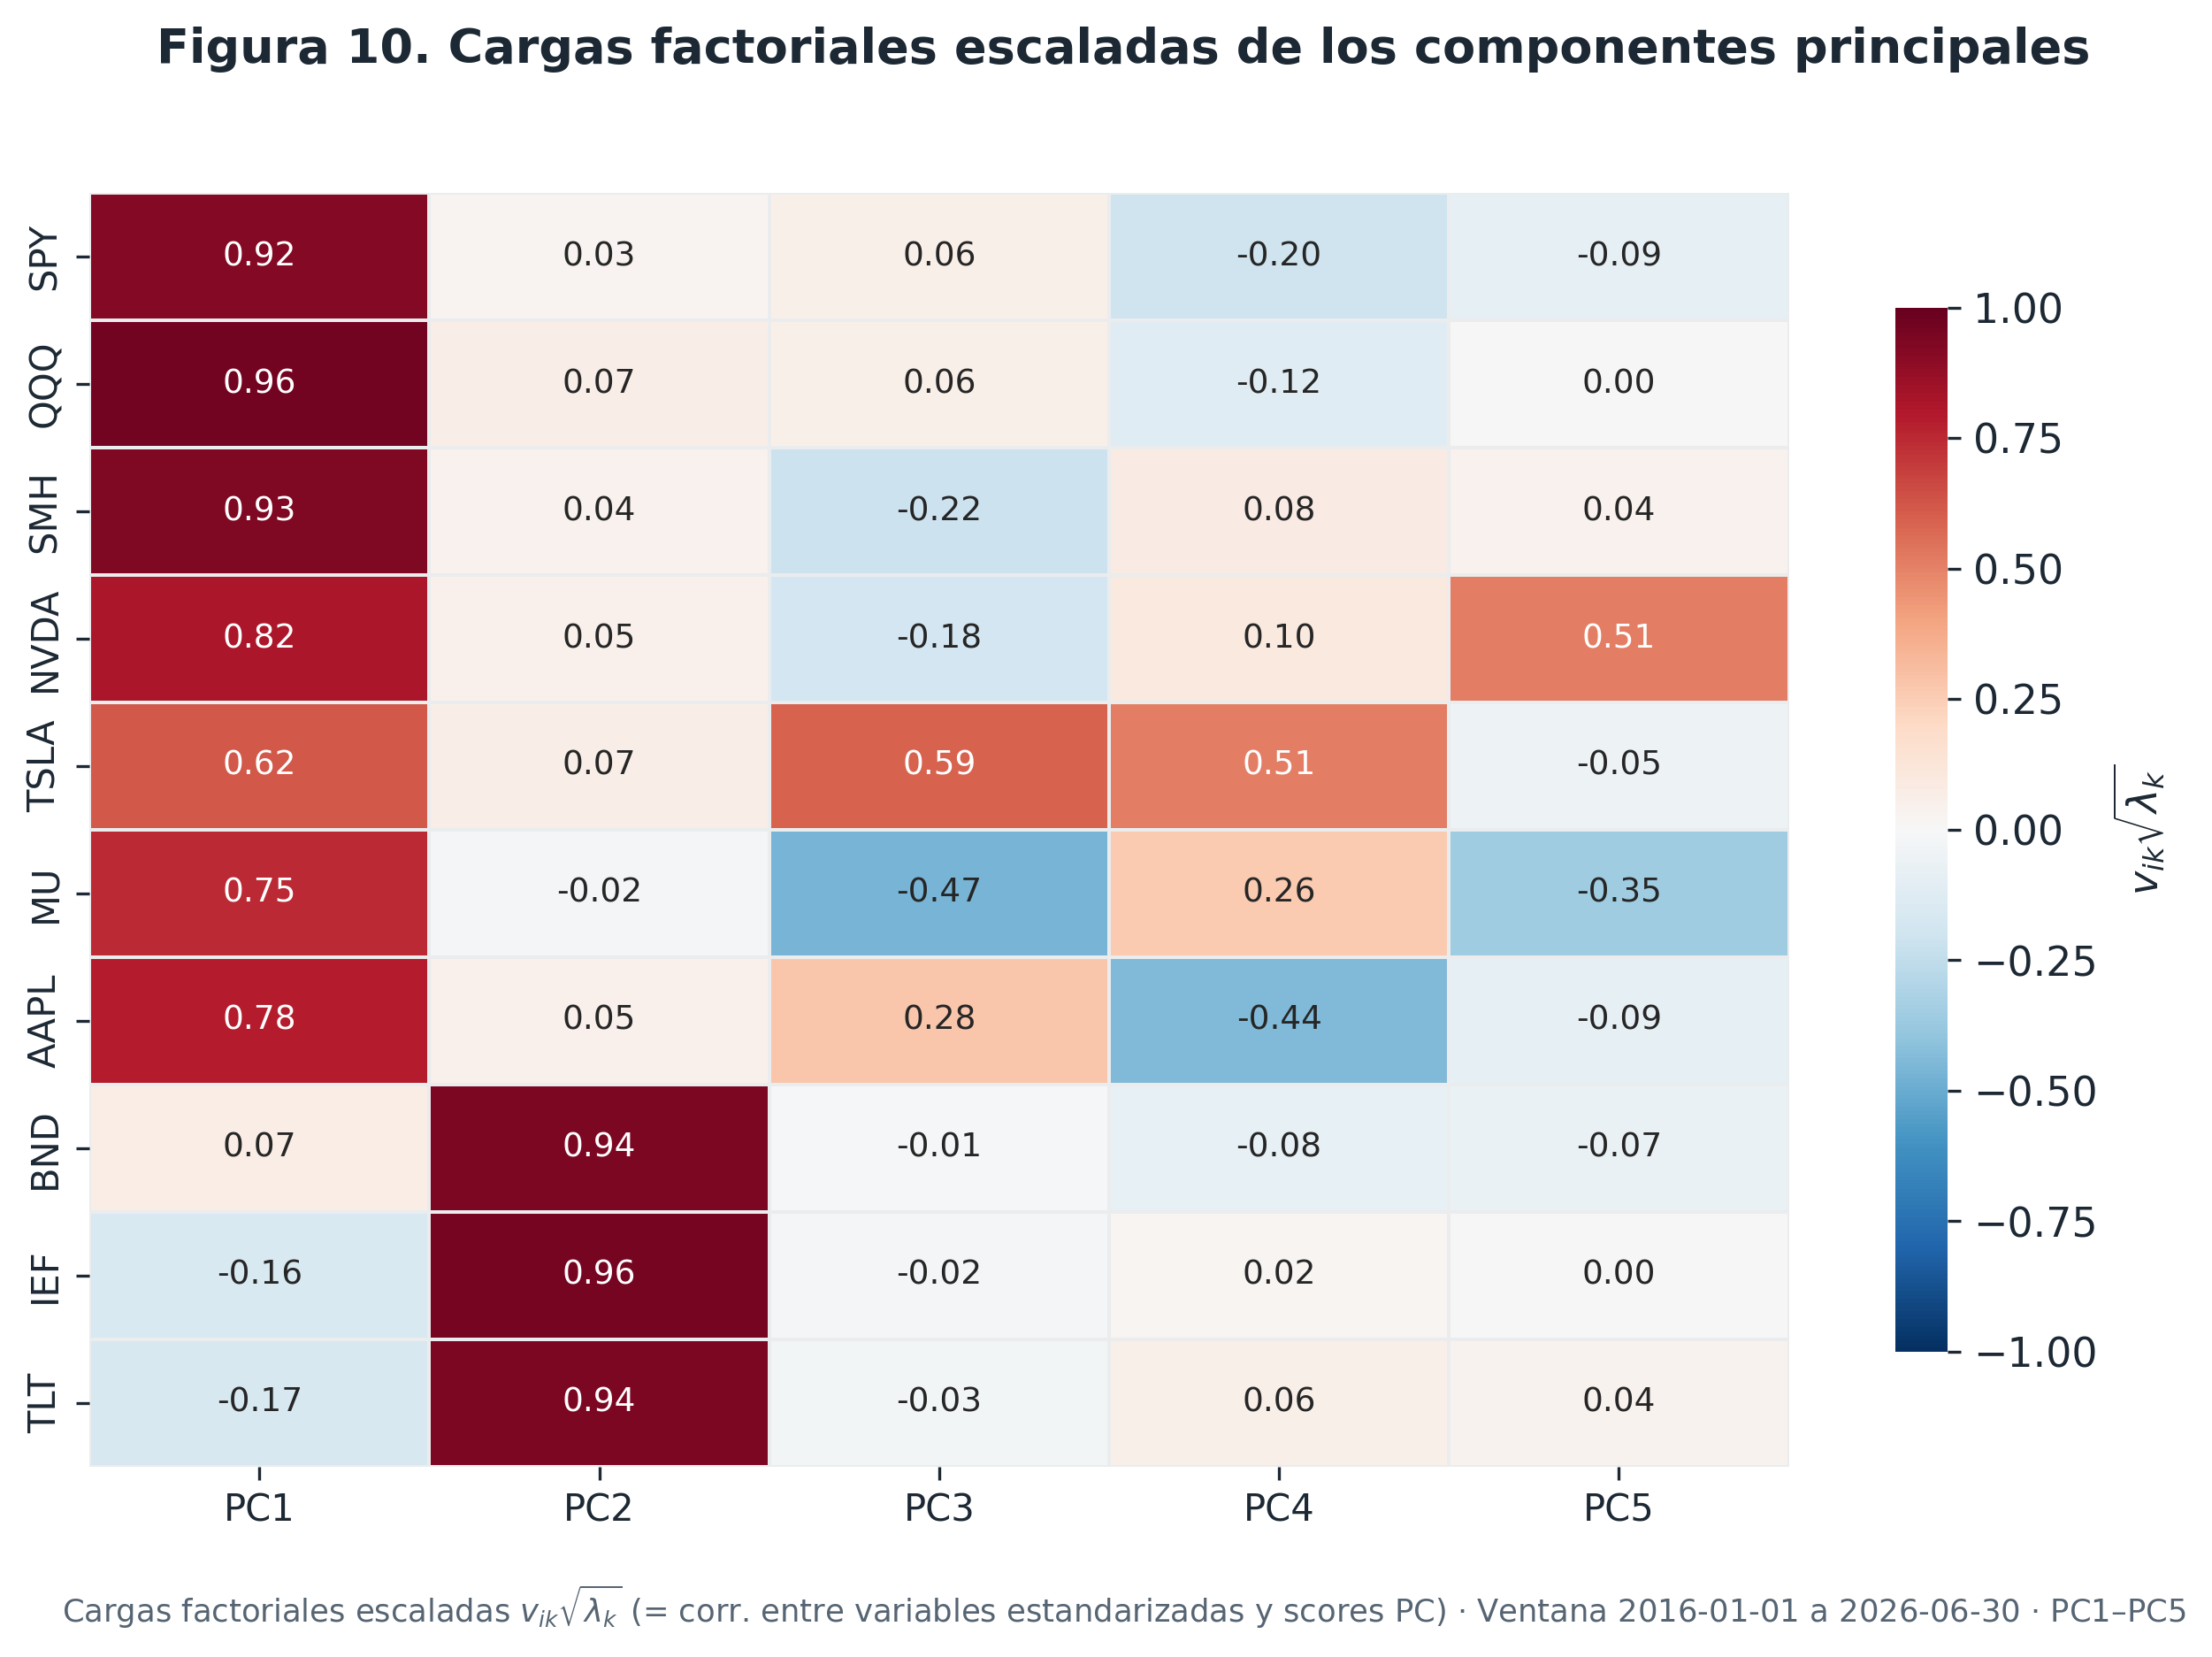
\includegraphics[width=0.92\textwidth]{fig10_pca_loadings_es.png}
\caption{Loadings escalados \(v_{ik}\sqrt{\lambda_k}\) (correlación entre variables estandarizadas y scores de los componentes).}
\end{figure}

La Figura~10 reporta loadings escalados, no eigenvectors puros. Cualquier lectura económica debe derivarse del patrón observado. PC1 muestra correlaciones elevadas con el bloque de renta variable; PC2 concentra correlaciones altas con BND, IEF y TLT. Ese contraste motiva, con cautela, asociar PC1 a una fuente común dominada por renta variable y PC2 a una dominada por renta fija, sin postularlos como factores observables exógenos. Tres componentes alcanzan el 80\% y cinco el 90\% de la variabilidad conjunta.

Hasta aquí, el diagnóstico avanzó midiendo posiciones, pesos, correlaciones y contribuciones al riesgo. El PCA cambia el plano de la pregunta. Ya no se pregunta únicamente \emph{cuántos activos} contiene la cartera, sino \emph{cuántas fuentes relativamente independientes explican su comportamiento conjunto}. En la muestra analizada, diez instrumentos no equivalen a diez dimensiones de variación: la mayor parte de la estructura común se concentra en un número reducido de componentes. Ese resultado no ``optimiza'' el portafolio; revela que la diversificación aparente por conteo puede coexistir con una dependencia factorial elevada. En la definición adoptada en este trabajo ---múltiples fuentes relativamente independientes de riesgo---, el PCA es, por tanto, el cierre conceptual del diagnóstico: traduce la intuición de ``muchos tickers'' a una métrica de dimensionalidad efectiva del riesgo conjunto.

% ========================= 8. AUTOPSIA =========================
\section{La autopsia del portafolio}

Las capas anteriores pueden leerse por separado. Integradas, constituyen la autopsia del portafolio: un recorrido que parte del conteo nominal y termina en las fuentes comunes de variación.

\begin{center}
\large
10 activos nominales\\[0.35em]
$\downarrow$\\[0.35em]
9{,}55 posiciones efectivas por capital\\[0.35em]
$\downarrow$\\[0.35em]
6{,}58 posiciones efectivas por riesgo\\[0.35em]
$\downarrow$\\[0.35em]
3 fuentes comunes dominantes ($\ge 80\%$ de la variabilidad conjunta)
\end{center}

\vspace{0.6em}

\begin{table}[H]
\centering
\small
\begin{tabular}{lc}
\toprule
Dimensión & Resultado \\
\midrule
Número nominal de activos & 10 \\
Effective Positions by Capital & 9{,}55 \\
Effective Positions by Risk & 6{,}58 \\
Componentes para explicar $\ge 80\%$ (PCA) & 3 \\
Componentes para explicar $\ge 90\%$ (PCA) & 5 \\
\bottomrule
\end{tabular}
\caption{Integración de las capas del diagnóstico.}
\end{table}

\begin{figure}[H]
\centering
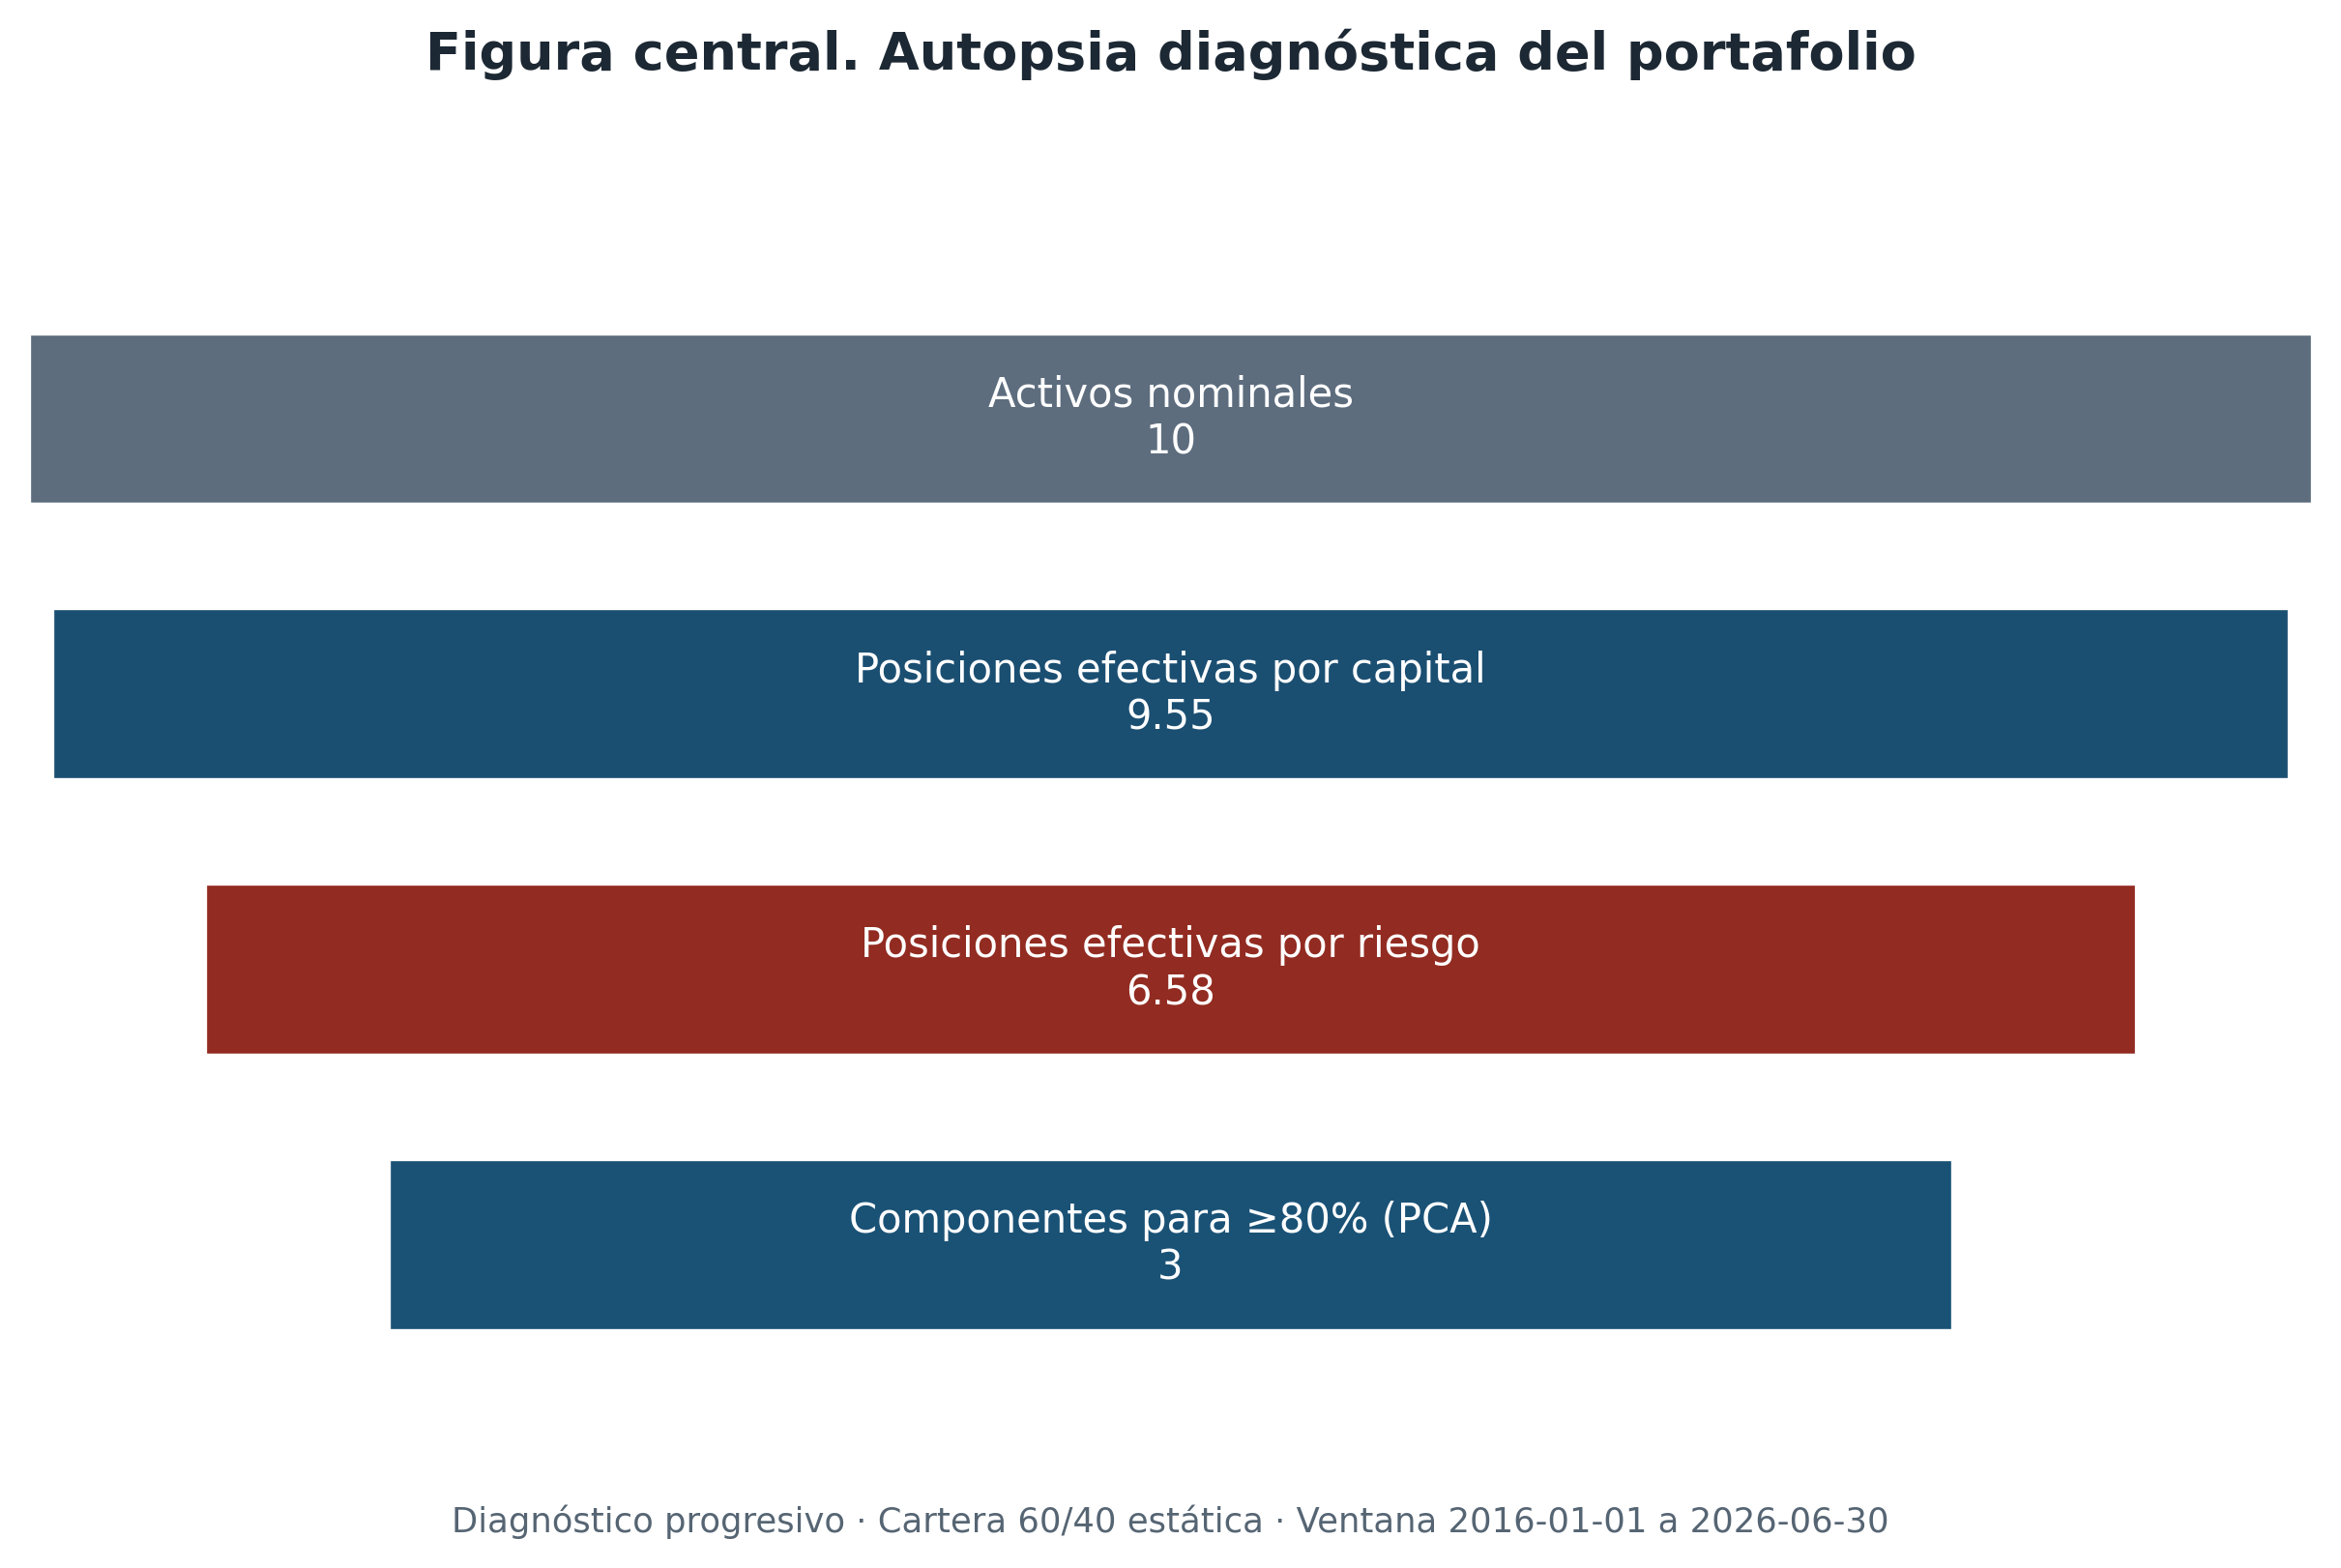
\includegraphics[width=0.82\textwidth]{fig_central_autopsia_es.png}
\caption{Autopsia diagnóstica del portafolio.}
\end{figure}

La contracción es leve cuando se mide capital y marcada cuando se mide riesgo; en el plano factorial, tres componentes bastan para explicar al menos el 80\% de la variabilidad conjunta. Respecto del conteo nominal de diez instrumentos, ello implica que la cartera \emph{pierde} el 70\% de sus fuentes aparentemente independientes de diversificación durante la autopsia: de diez activos contados a tres dimensiones dominantes de variación común. El resultado no niega el rol diversificador de la separación entre clases; muestra que el número de tickers sobredimensiona la independencia efectiva del portafolio.

% ========================= 9. CONCLUSIONES =========================
\section{Conclusiones}

La pregunta de investigación era: \textquestiondown{}hasta qué punto el número de activos de una cartera refleja su grado efectivo de diversificación?

Sobre la cartera 60/40 analizada (2016-01-01 a 2026-06-30), la evidencia empírica indica que el conteo nominal es una medida insuficiente.

\begin{enumerate}
\item \textbf{Capital.} Con \(N=10\), \(N_{\mathrm{eff,weights}}=9{,}55\): no se observa concentración material del capital a partir de los pesos objetivo.
\item \textbf{Dependencia.} Las correlaciones son elevadas dentro de cada clase y bajas entre clases: diez tickers no equivalen a diez comportamientos independientes.
\item \textbf{Riesgo.} La renta variable concentra el 97{,}65\% de la contribución total al riesgo; TSLA, NVDA y MU dominan el PRC pese a pesos idénticos al resto del bloque equity.
\item \textbf{Posiciones efectivas.} Al pasar de capital a PRC, \(N_{\mathrm{eff}}\) cae de 9{,}55 a 6{,}58.
\item \textbf{Fuentes comunes.} El PCA identifica 3 componentes para \(\ge 80\%\) y 5 para \(\ge 90\%\) de la variabilidad conjunta.
\end{enumerate}

\paragraph{Conclusión conceptual.}
La diversificación ---entendida aquí como la existencia de múltiples fuentes relativamente independientes de riesgo--- no puede evaluarse exclusivamente contando activos. El error cognitivo de igualar cantidad de instrumentos con diversificación queda rechazado por la evidencia de esta cartera. El diagnóstico requiere analizar la dependencia entre instrumentos, la distribución de las contribuciones al riesgo y la estructura de factores comunes que explican su comportamiento conjunto.

El estudio es diagnóstico, no normativo: no optimiza la cartera ni prescribe una asignación alternativa.

\end{document}
